%\documentclass[ba]{imsart}
%% use command below for supplement
 \documentclass[ba,preprint]{imsart}
%
\pubyear{2023}
\volume{TBA}
\issue{TBA}
% \doi{0000}
%\arxiv{}
\firstpage{1}
\lastpage{1}

\usepackage{lineno}
\usepackage{amsthm}
\usepackage{amsmath}
\usepackage{natbib}
\usepackage[colorlinks,citecolor=blue,urlcolor=blue,filecolor=blue,backref=page]{hyperref}
\usepackage{graphicx}
\newtheorem{lemma}{Lemma}
\newtheorem{example}{Example}
\newtheorem{rem}{Remark}
\usepackage{booktabs}       % professional-quality tables
\usepackage{algorithm}      % algorithm environment
\usepackage{algpseudocode}
\usepackage{subcaption}
\usepackage{soul}

\startlocaldefs
\setbeamertemplate{navigation symbols}{}
\setbeamertemplate{footline}[page number]
\endlocaldefs

%%% only for appendix
\renewcommand{\appendixname}{Supplement}
%%%




%%% start code for cross referencing main document with the appendix %%

\usepackage{xr} %%(must be loaded before hyperref) and I found an example of this on Overleaf that was extremely helpful

\makeatletter

\newcommand*{\addFileDependency}[1]{% argument=file name and extension
\typeout{(#1)}% latexmk will find this if $recorder=0
% however, in that case, it will ignore #1 if it is a .aux or 
% .pdf file etc and it exists! If it doesn't exist, it will appear 
% in the list of dependents regardless)
%
% Write the following if you want it to appear in \listfiles 
% --- although not really necessary and latexmk doesn't use this
%
\@addtofilelist{#1}
%
% latexmk will find this message if #1 doesn't exist (yet)
\IfFileExists{#1}{}{\typeout{No file #1.}}
}\makeatother

\newcommand*{\myexternaldocument}[1]{%
\externaldocument{#1}%
\addFileDependency{#1.tex}%
\addFileDependency{#1.aux}%
}
%------------End of helper code--------------

% put all the external documents here!
\myexternaldocument{main4}
%% To run this you must run the compiler through pdflatexmk and have the latexmkrc file within the folder

%%% end code for cross referencing main document with the appendix %%

\begin{document}

%% *** Frontmatter *** 
\linenumbers
\begin{frontmatter}
\title{Supplementary Material for ``Efficient and Scalable Bipartite Matching with Fast Beta Linkage  (fabl)"}
%\title{A Sample Document\thanksref{T1}}
%\thankstext{T1}{<thanks text>}
\runtitle{Efficient and Scalable Bipartite Matching with Fast Beta Linkage  (fabl)}

\begin{aug}
\author{\fnms{Brian} \snm{Kundinger}\thanksref{addr1}\ead[label=e1]{brian.kundinger@duke.edu}},
\author{\fnms{Jerome P.} \snm{Reiter}\thanksref{addr1}\ead[label=e2]{jreiter@duke.edu}}
\and
\author{\fnms{Rebecca C.} \snm{Steorts}\thanksref{addr1}\ead[label=e3]{beka@stat.duke.edu}}

\runauthor{Kundinger et al.}

\address[addr1]{Department of Statistical Science,
Duke University,
P.O.\ Box 90251,
Durham, NC 27708, USA
\printead{e1}, % print email address of "e1"
\printead*{e2},
\printead*{e3}
}

%\address[addr2]{Departments of Statistical Science and Computer Science,
%Duke University,
%P.O.\ Box 90251,
%Durham, NC 27708, USA
%\printead{e3}
%}

%\thankstext{<id>}{<text>}
\end{aug}






\end{frontmatter}


	

\appendix
	
		
	\hypertarget{app:derivations}{%
		\section{Derivations of Full Conditionals}\label{app:derivations}}
	
	We provide detailed derivations of the full conditionals provided in Section \ref{sec:fast-beta-linkage} in the main text. The $\bm{m}$ and $\bm{u}$ parameters are updated through standard multinomial-Dirichlet distributions. For a particular $m_{fl}$, we have
	\begin{align}
		\mathcal{L}(m_{fl}|\gamma, \bm{u}, \bm{Z}, \pi) &\propto \prod_{i=1}^{n_A} \prod_{j=1}^{n_B} m_{fl}^{I(Z_j = i) I(\gamma_{ij}^f = l) I_{obs}(\gamma_{ij}^f)}  m_{fl}^{\alpha_{fl} - 1} = m_{fl}^{\alpha_{fl}(\bm{Z}) - 1},
	\end{align}
	where $\alpha_{fl}(\bm{Z})= \alpha_{fl} + \sum_{i=1}^{n_A}  \sum_{j=1}^{n_B} I_{obs}(\gamma_{ij}^f)I(\gamma_{ij}^f = l) I(Z_j = i)$. Analogous procedures lead to $\mathcal{L}(u_{fl}| \gamma, \bm{m}, \bm{Z}, \pi)$  $\propto u_{fl}^{\beta_{fl}(\bm{Z}) - 1}$, where $\beta_{fl}(\bm{Z})= \beta_{fl} + \sum_{i=1}^{n_A}  \sum_{j=1}^{n_B} I_{obs}(\gamma_{ij}^f)I(\gamma_{ij}^f = l) I(Z_j \neq i)$. Thus, for the vectors of parameters $\bm{m}_f$ and $\bm{u}_f$, we have
	\begin{align}
	\bm{m}_f^{(s+1)} |
	\gamma, 
	\bm{Z}^{(s)}, \bm{u}^{(s)}, \pi^{(s)} &\sim 
	\text{Dirichlet}(\alpha_{f1}(\bm{Z}^{(s)}), \ldots, \alpha_{fL_f}(\bm{Z}^{(s)})), \\
	\bm{u}_f^{(s+1)} | \gamma, \bm{Z}^{(s)}, \bm{m}^{(s)}, \pi^{(s)} &\sim \text{Dirichlet}(\beta_{f1}(\bm{Z}^{(s)}), \ldots, \beta_{fL_f}(\bm{Z}^{(s)})).
	\end{align}

	Since $\pi$ encodes the rate of matching across the two data files, the full conditional $p(\pi|\gamma, \bm{Z}, \bm{m}, \bm{u}, \alpha_{\pi}, \beta_{\pi})$ depends only on the number of links $n_{AB}(\bm{Z}) = \sum_{j=1}^{n_B}I(Z_j \leq n_A)$ encoded by $\bm{Z}$ and hyperparameters. We have the full conditional
	\begin{align}
		p(\pi |\gamma, \bm{Z}, \bm{m}, \bm{u}) &\propto p(\bm{Z}|\pi)p(\pi) \\
		&\propto \pi^{n_{AB}(\bm{Z})} (1-\pi)^{n_B - n_{AB}(\bm{Z})} \pi^{\alpha_{\pi} -1} (1-\pi)^{\beta_{\pi} -1} \\
		&\propto \pi^{n_{AB}(\bm{Z}) + \alpha_{\pi} - 1} (1-\pi)^{n_A - n_{AB}(\bm{Z}) + \beta_{\pi} -1}.
	\end{align}
	Thus, $\pi^{(s+1)}|\gamma, \bm{Z}^{(s)}, \bm{m}^{(s+1)}, \bm{u}^{(s+1)}$ has a $\text{Beta}(n_{AB}(\bm{Z}^{(s)}) + \alpha_{\pi}, n_B - n_{AB}(\bm{Z}^{(s)}) + \beta_{\pi})$ distribution.
	
	Due to the independence in the fast beta prior in \eqref{eqn:fast_beta_prior}, we can obtain the full conditional for $\bm{Z}$ through the full conditionals for each individual $Z_j$. Let $\Gamma_{.j}$ denote the random matrix of $n_A$ comparison vectors relating to an arbitrary record $B_j$, and let $\gamma_{.j}$ be a realization of $\Gamma_{.j}$. We have
	\begin{align}
		p(\bm{Z} | \gamma, \bm{m}, \bm{u}, \pi) &= \prod_{j=1}^{n_B} p(Z_j | \gamma_{.j}, \bm{m}, \bm{u}, \pi).
		%&\propto p(\Gamma| \bm{Z}, \bm{m}, \bm{u}) p(\bm{Z} | \pi) \\
		%&=\prod_{j=1}^{n_B} p(\Gamma_{.j}| Z_j, \bm{m}, \bm{u}) p(Z_j | \pi) \\
	\end{align}
{
\color{blue}{
Following the observation of \cite{wortman2019}, when $B_j$ does not link to any record in $A$, the contribution to the likelihood is simply a product of $u$ parameters, which we will call $c_j$:
\begin{align}
	p(\Gamma_{.j}| \bm{m}, \bm{u}, \pi, Z_j = n_A + j) = \prod_{i=1}^{n_A}\prod_{f=1}^{F}\prod_{l=1}^{L_f} u_{fl}^{I(\gamma_{ij}^f = l)I_{obs}(\gamma_{ij}^f)} = c_j.
\end{align}
When $Z_j = q$ for some $q\leq n_A$, we have
\begin{align}
	p(\Gamma_{.j}| \bm{m}, \bm{u}, \pi,  Z_j = q) =\prod_{f=1}^{F}\prod_{l=1}^{L_f} m_{fl}^{I(\gamma_{qj}^f = l)I_{obs}(\gamma_{qj}^f)}  \prod_{i \neq q}\prod_{f=1}^{F}\prod_{l=1}^{L_f} u_{fl}^{I(\gamma_{ij}^f = l)I_{obs}(\gamma_{ij}^f)}.
\end{align}
We multiply and divide by the $u$ parameters for the matching record pair to obtain
\begin{align}
	p(\Gamma_{.j}| \bm{m}, \bm{u}, \pi, Z_j = q) &= \prod_{f=1}^{F}\prod_{l=1}^{L_f} \left(\frac{m_{fl}}{u_{fl}}\right)^{I(\gamma_{qj}^f = l)I_{obs}(\gamma_{qj}^f)}  \prod_{i = 1}^{n_A}\prod_{f=1}^{F}\prod_{l=1}^{L_f} u_{fl}^{I(\gamma_{ij}^f = l)I_{obs}(\gamma_{ij}^f)} \\
	&= w_{qj}  c_j.
\end{align}
We can divide the result of each case by $c_j$ to get
\begin{align}
	p(\Gamma_{.j}| \bm{m}, \bm{u}, \pi, Z_j) \propto \begin{cases} 
		w_{qj}, & q \leq n_A; \\
		1, &  q  = n_A + j.
	\end{cases}
\end{align}
Lastly, we multiply the likelihood by the fast beta prior in (\ref{eqn:fast_beta_prior}) to obtain the full conditional
\begin{align}
	\label{eqn:z_full_conditional2}
	p\left(Z_j^{(s+1)}  = q|\gamma, \bm{m}^{(s+1)}, \bm{u}^{(s+1)}, \pi^{(s+1)}\right) \propto
	\begin{cases} 
		\frac{\pi^{(s+1)}}{n_A} w_{qj}^{(s+1)},  & q \leq n_A; \\
		1 - \pi^{(s+1)}, & q  = n_A + j.
	\end{cases}
\end{align}
}
}

{
\color{red}{Following the observation of \cite{wortman2019}, when $B_j$ does not link to any record in $A$, the contribution to the likelihood is simply a product of $u$ parameters, which we will call $c_j$:
	\begin{align}
		\mathcal{L}(Z_j = n_A + j| \bm{m}, \bm{u}, \pi, \Gamma_{.j}) = \prod_{i=1}^{n_A}\prod_{f=1}^{F}\prod_{l=1}^{L_f} u_{fl}^{I(\gamma_{ij}^f = l)I_{obs}(\gamma_{ij}^f)} = c_j.
	\end{align}
	When $Z_j = q$ for some $q\leq n_A$, we have
	\begin{align}
		\mathcal{L}(Z_j = q| \bm{m}, \bm{u}, \pi, \Gamma_{.j}) =\prod_{f=1}^{F}\prod_{l=1}^{L_f} m_{fl}^{I(\gamma_{qj}^f = l)I_{obs}(\gamma_{qj}^f)}  \prod_{i \neq q}\prod_{f=1}^{F}\prod_{l=1}^{L_f} u_{fl}^{I(\gamma_{ij}^f = l)I_{obs}(\gamma_{ij}^f)}.
	\end{align}
	We multiply and divide by the $u$ parameters for the matching record pair to obtain
	\begin{align}
		\mathcal{L}(Z_j = q| \bm{m}, \bm{u}, \pi, \Gamma_{.j}) &= \prod_{f=1}^{F}\prod_{l=1}^{L_f} \left(\frac{m_{fl}}{u_{fl}}\right)^{I(\gamma_{qj}^f = l)I_{obs}(\gamma_{qj}^f)}  \prod_{i = 1}^{n_A}\prod_{f=1}^{F}\prod_{l=1}^{L_f} u_{fl}^{I(\gamma_{ij}^f = l)I_{obs}(\gamma_{ij}^f)} \\
		&= w_{qj}  c_j.
	\end{align}
	We can divide the result of each case by $c_j$ to get
	\begin{align}
		\mathcal{L}(Z_j | \bm{m}, \bm{u}, \pi, \Gamma_{.j}) \propto \begin{cases} 
			w_{qj}, & q \leq n_A; \\
			1, &  q  = n_A + j.
		\end{cases}
	\end{align}
	Lastly, we multiply the likelihood by the fast beta prior in (\ref{eqn:fast_beta_prior}) to obtain the full conditional
	\begin{align}
		\label{eqn:z_full_conditional2}
		p\left(Z_j^{(s+1)}  = q|\gamma, \bm{m}^{(s+1)}, \bm{u}^{(s+1)}, \pi^{(s+1)}\right) \propto
		\begin{cases} 
			\frac{\pi^{(s+1)}}{n_A} w_{qj}^{(s+1)},  & q \leq n_A; \\
			1 - \pi^{(s+1)}, & q  = n_A + j.
		\end{cases}
	\end{align}
}
}

	
%	To express the full conditional for $\bm{Z}$, we consider the cases where $Z_j$ does not have a link in $A$ and where $Z_j$ does have a link in $A$. Because we sample each $Z_j$ independently of all other $Z_{j'}$ (for $j \neq j'$), we need only the full conditional for each individual $Z_j$. Let $\Gamma_{.j}$ denote the matrix of $n_A$ comparison vectors relating to record $B_j$. Following the observation of \cite{wortman2019}, when $B_j$ does not link to any record in $A$, the contribution to the likelihood is simply a product of $u$ parameters, which we will call $c_j$:
%	\begin{align}
%		p(\Gamma_{.j}| \bm{m}, \bm{u}, \pi, Z_j = n_A + j) = \prod_{i=1}^{n_A}\prod_{f=1}^{F}\prod_{l=1}^{L_f} u_{fl}^{I(\gamma_{ij}^f = l)I_{obs}(\gamma_{ij}^f)} = c_j.
%	\end{align}
%	When $Z_j = q$ for some $q\leq n_A$, we have
%	\begin{align}
%		p(\Gamma_{.j}| \bm{m}, \bm{u}, \pi,  Z_j = q) =\prod_{f=1}^{F}\prod_{l=1}^{L_f} m_{fl}^{I(\gamma_{qj}^f = l)I_{obs}(\gamma_{qj}^f)}  \prod_{i \neq q}\prod_{f=1}^{F}\prod_{l=1}^{L_f} u_{fl}^{I(\gamma_{ij}^f = l)I_{obs}(\gamma_{ij}^f)}.
%	\end{align}
%	We multiply and divide by the $u$ parameters for the matching record pair to obtain
%	\begin{align}
%		p(\Gamma_{.j}| \bm{m}, \bm{u}, \pi, Z_j = q) &= \prod_{f=1}^{F}\prod_{l=1}^{L_f} \left(\frac{m_{fl}}{u_{fl}}\right)^{I(\gamma_{qj}^f = l)I_{obs}(\gamma_{qj}^f)}  \prod_{i = 1}^{n_A}\prod_{f=1}^{F}\prod_{l=1}^{L_f} u_{fl}^{I(\gamma_{ij}^f = l)I_{obs}(\gamma_{ij}^f)} \\
%		&= w_{qj}  c_j.
%	\end{align}
%	We can divide the result of each case by $c_j$ to get
%	\begin{align}
%		p(\Gamma_{.j}| \bm{m}, \bm{u}, \pi, Z_j) \propto \begin{cases} 
%			w_{qj}, & q \leq n_A; \\
%			1, &  q  = n_A + j. \
%		\end{cases}
%	\end{align}
%	Lastly, we multiply the likelihood by the fast beta prior in (\ref{eqn:fast_beta_prior}) to obtain the full conditional
%	\begin{align}
%		\label{eqn:z_full_conditional2}
%		p\left(Z_j^{(s+1)}  = q|\gamma, \bm{m}^{(s+1)}, \bm{u}^{(s+1)}, \pi^{(s+1)}\right) \propto
%		\begin{cases} 
%			\frac{\pi^{(s+1)}}{n_A} w_{qj}^{(s+1)},  & q \leq n_A; \\
%			1 - \pi^{(s+1)}, & q  = n_A + j. \
%		\end{cases}
%	\end{align}
	
	\hypertarget{bayes-estimate}{%
		\section{Bayes Estimate}
		\label{bayes-estimate}}
	
We calculate a Bayes estimate $\hat{\bm{Z}}$ for the linkage parameter $\bm{Z}$ by assigning different positive losses to different types of errors, and minimizing posterior expected loss. We adopt the loss function proposed in \cite{sadinle_bayesian_2017} in which $\hat{Z}_j \in \{1, \ldots, n_A, n_A + j, R\}$, with $R$ representing the option to leave the matching undetermined by the model. Specifically, we have
\begin{align}
	L(\hat{Z_j}, Z_j)=\begin{cases} 
		0,  & \text{if } Z_j = \hat{Z_j}; \\
		\theta_R,  & \text{if } \hat{Z_j} = R; \\
		\theta_{10},  & \text{if } Z_j \leq 1,\hat{Z_j} = n_A + j ; \\
		\theta_{01},  & \text{if } Z_j = n_A + j,\hat{Z_j} \leq n_A ; \\
		\theta_{11},  & \text{if } Z_j \leq n_A, \hat{Z}_j \leq n_A, Z_j \neq \hat{Z_j}. \\
	\end{cases}
\end{align}
Here, $\theta_R$ is the loss from not making a decision on the linkage status, $\theta_{10}$ is the loss from a false nonmatch, $\theta_{01}$ is the loss from a false match, and $\theta_{11}$ is the loss from the special case of a false match in which the record has a true match other than the one estimated by the model. 

In general, we follow \cite{sadinle_bayesian_2017} and set $(\theta_{10}, \theta_{01}, \theta_{11}, \theta_R) = (1, 1, 2, \infty)$ inducing the decision rule
	\begin{align}
		\hat{Z}_j =\begin{cases} 
		i,  & \text{if } p(Z_j = i |\gamma) > \frac{1}{2}; \\
		0,  & \text{otherwise}. \\
	\end{cases}
\end{align}
Since \texttt{fabl} does not strictly enforce one-to-one matching, it is possible for this Bayes estimate to link multiple records in $B$ to one record in $A$. In the event that we have two records $B_j$ and $B_{j'}$ such that both $p(\hat{Z}_j = i |\gamma) > \frac{1}{2}$ and $ p(\hat{Z}_{j'} = i |\gamma) > \frac{1}{2}$, we accept the match with the higher posterior probability, and declare the other to have no match. Since each $Z_j$ is independent, this is equivalent to minimizing the expected loss subject to the constraint that $\hat{Z}_j \neq \hat{Z}_{j'}$ for all $j \neq j'$.  A similar approach appears in the most probable maximal matching sets used by \cite{steorts_bayesian_2016} to match records to latent entities.

When we seek a partial estimate of the linkage structure, leaving a portion of record pairs to be classified manually in clerical review, we adopt losses $(\theta_{10}, \theta_{01}, \theta_{11}, \theta_R) = (1, 1, 2, .1)$. For a more in-depth explanation of this function and the induced Bayes estimate, see \cite{sadinle_bayesian_2017}.
	
	\hypertarget{appendix-sim}{%
		\section{Traceplots for Simulation Study}\label{app:appendix-sim}}
	Figures \ref{fig:sim_overlap_trace}, \ref{fig:sim_m_trace}, and \ref{fig:sim_u_trace} are traceplots for one of the 900 linkage tasks that comprise the simulation in Section \ref{accuracy} in the main text. It is set up with one error across the linkage fields and 50 duplicates across files. Traceplots across other settings exhibit similar behavior. Note that traceplots for $\bm{u}$ parameters show very little variation because the overwhelming majority of record pairs are nonmatching.  
	
	\begin{figure}[h]
		\begin{center}
			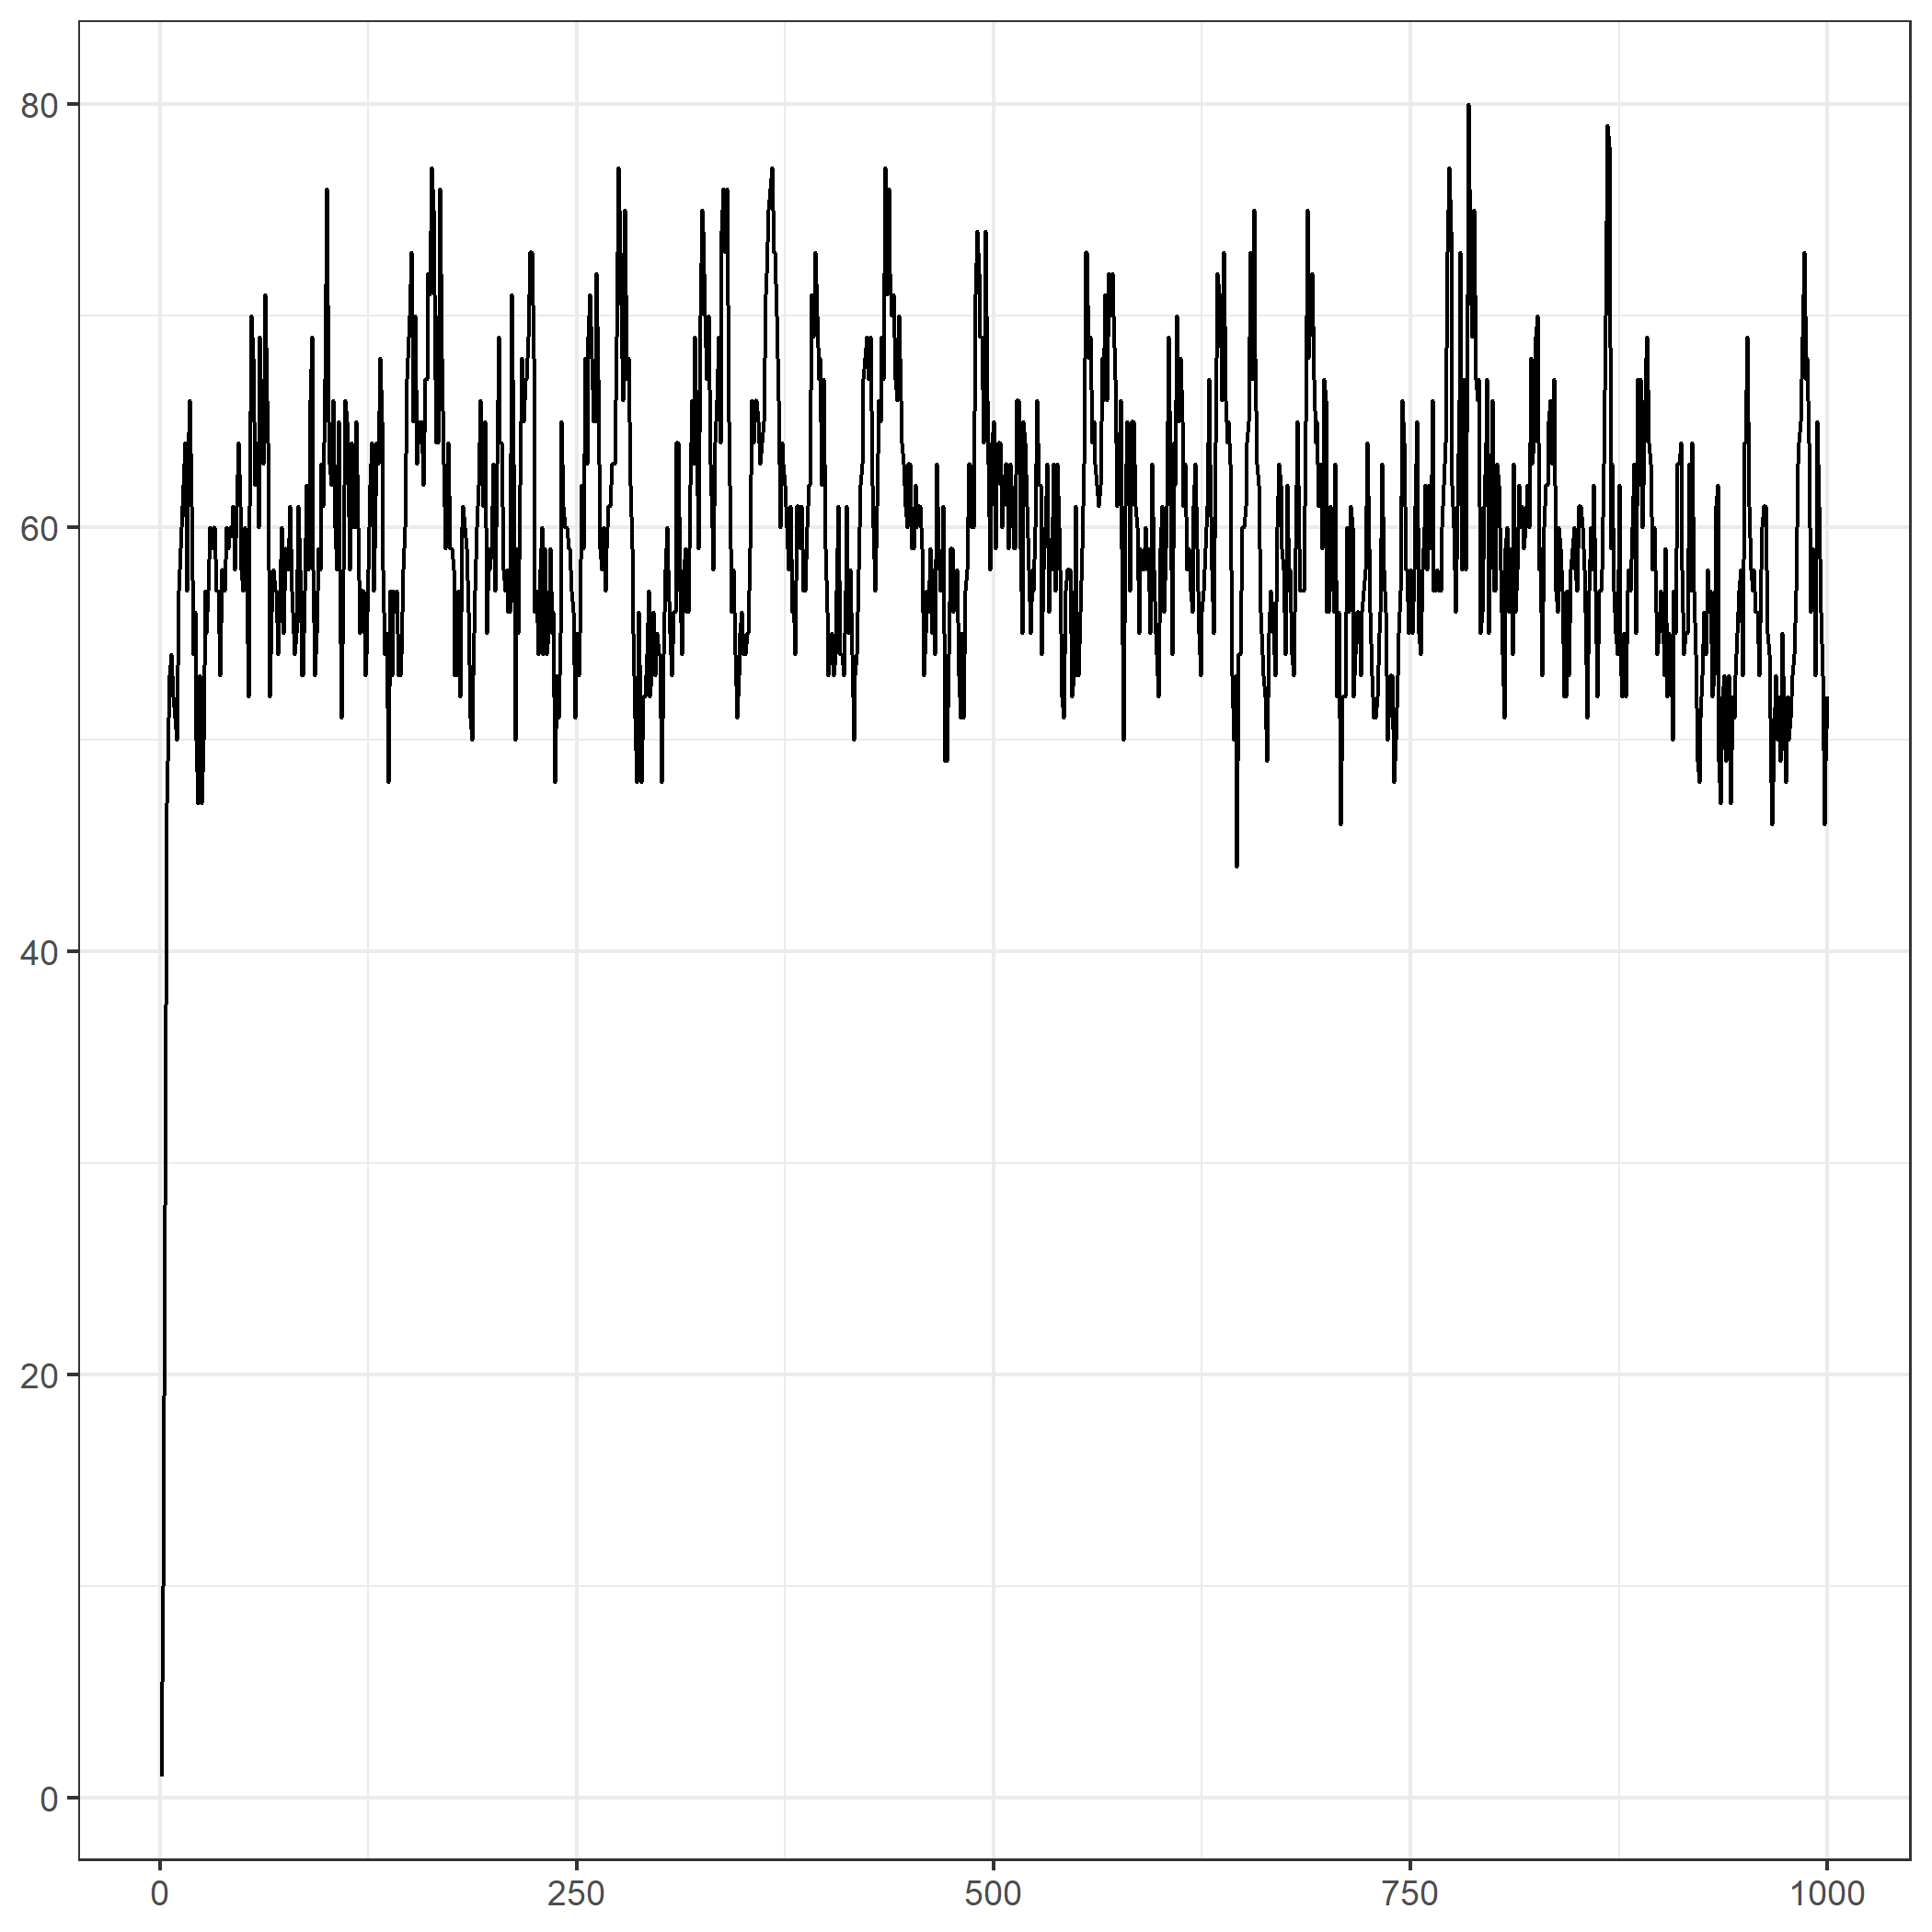
\includegraphics[width=0.6\textwidth]{../notes/figures/sim_overlap_trace} 
			\caption{Representative traceplot of overlap between files from simulation study in Section~\ref{accuracy} in the main text.} \label{fig:sim_overlap_trace}
		\end{center}
	\end{figure}
	
	
	\begin{figure}
		\begin{center}
			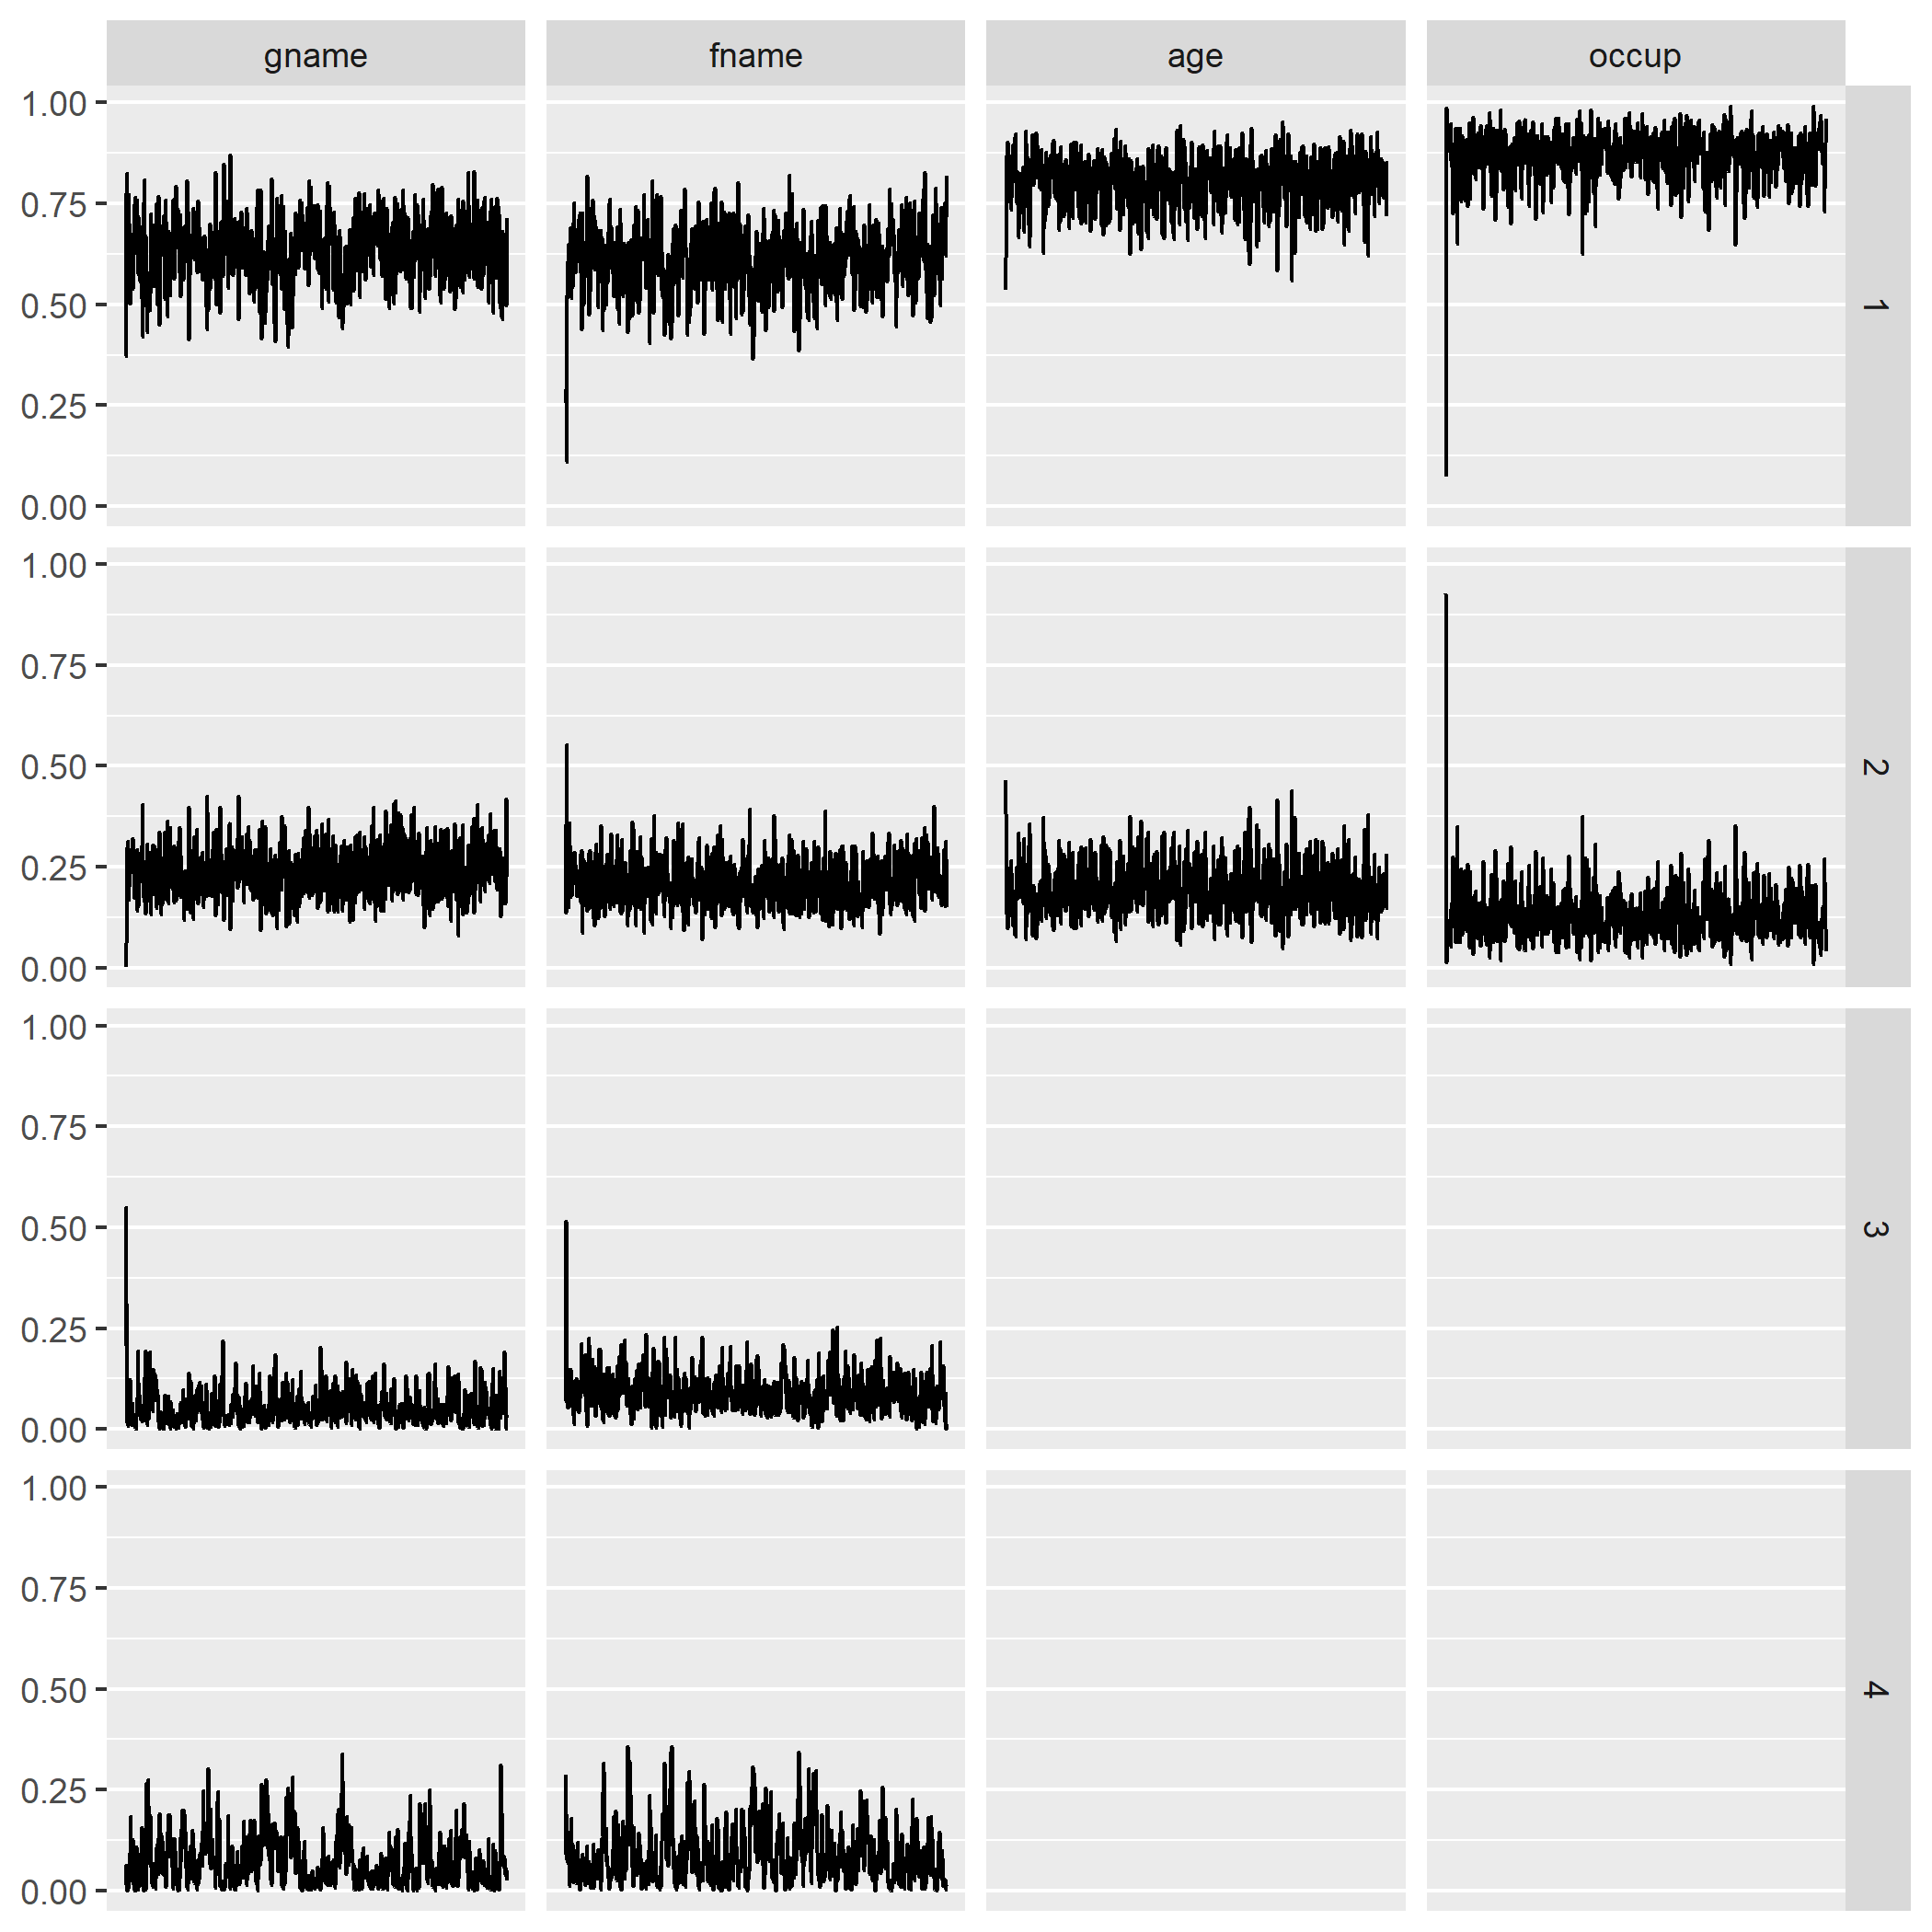
\includegraphics[width=0.6\textwidth]{../notes/figures/sim_m_trace} 
			\caption{Representative traceplot of $\bm{m}$ parameters from simulation study in Section~\ref{accuracy} in the main text.}\label{fig:sim_m_trace}
		\end{center}

		\begin{center}
			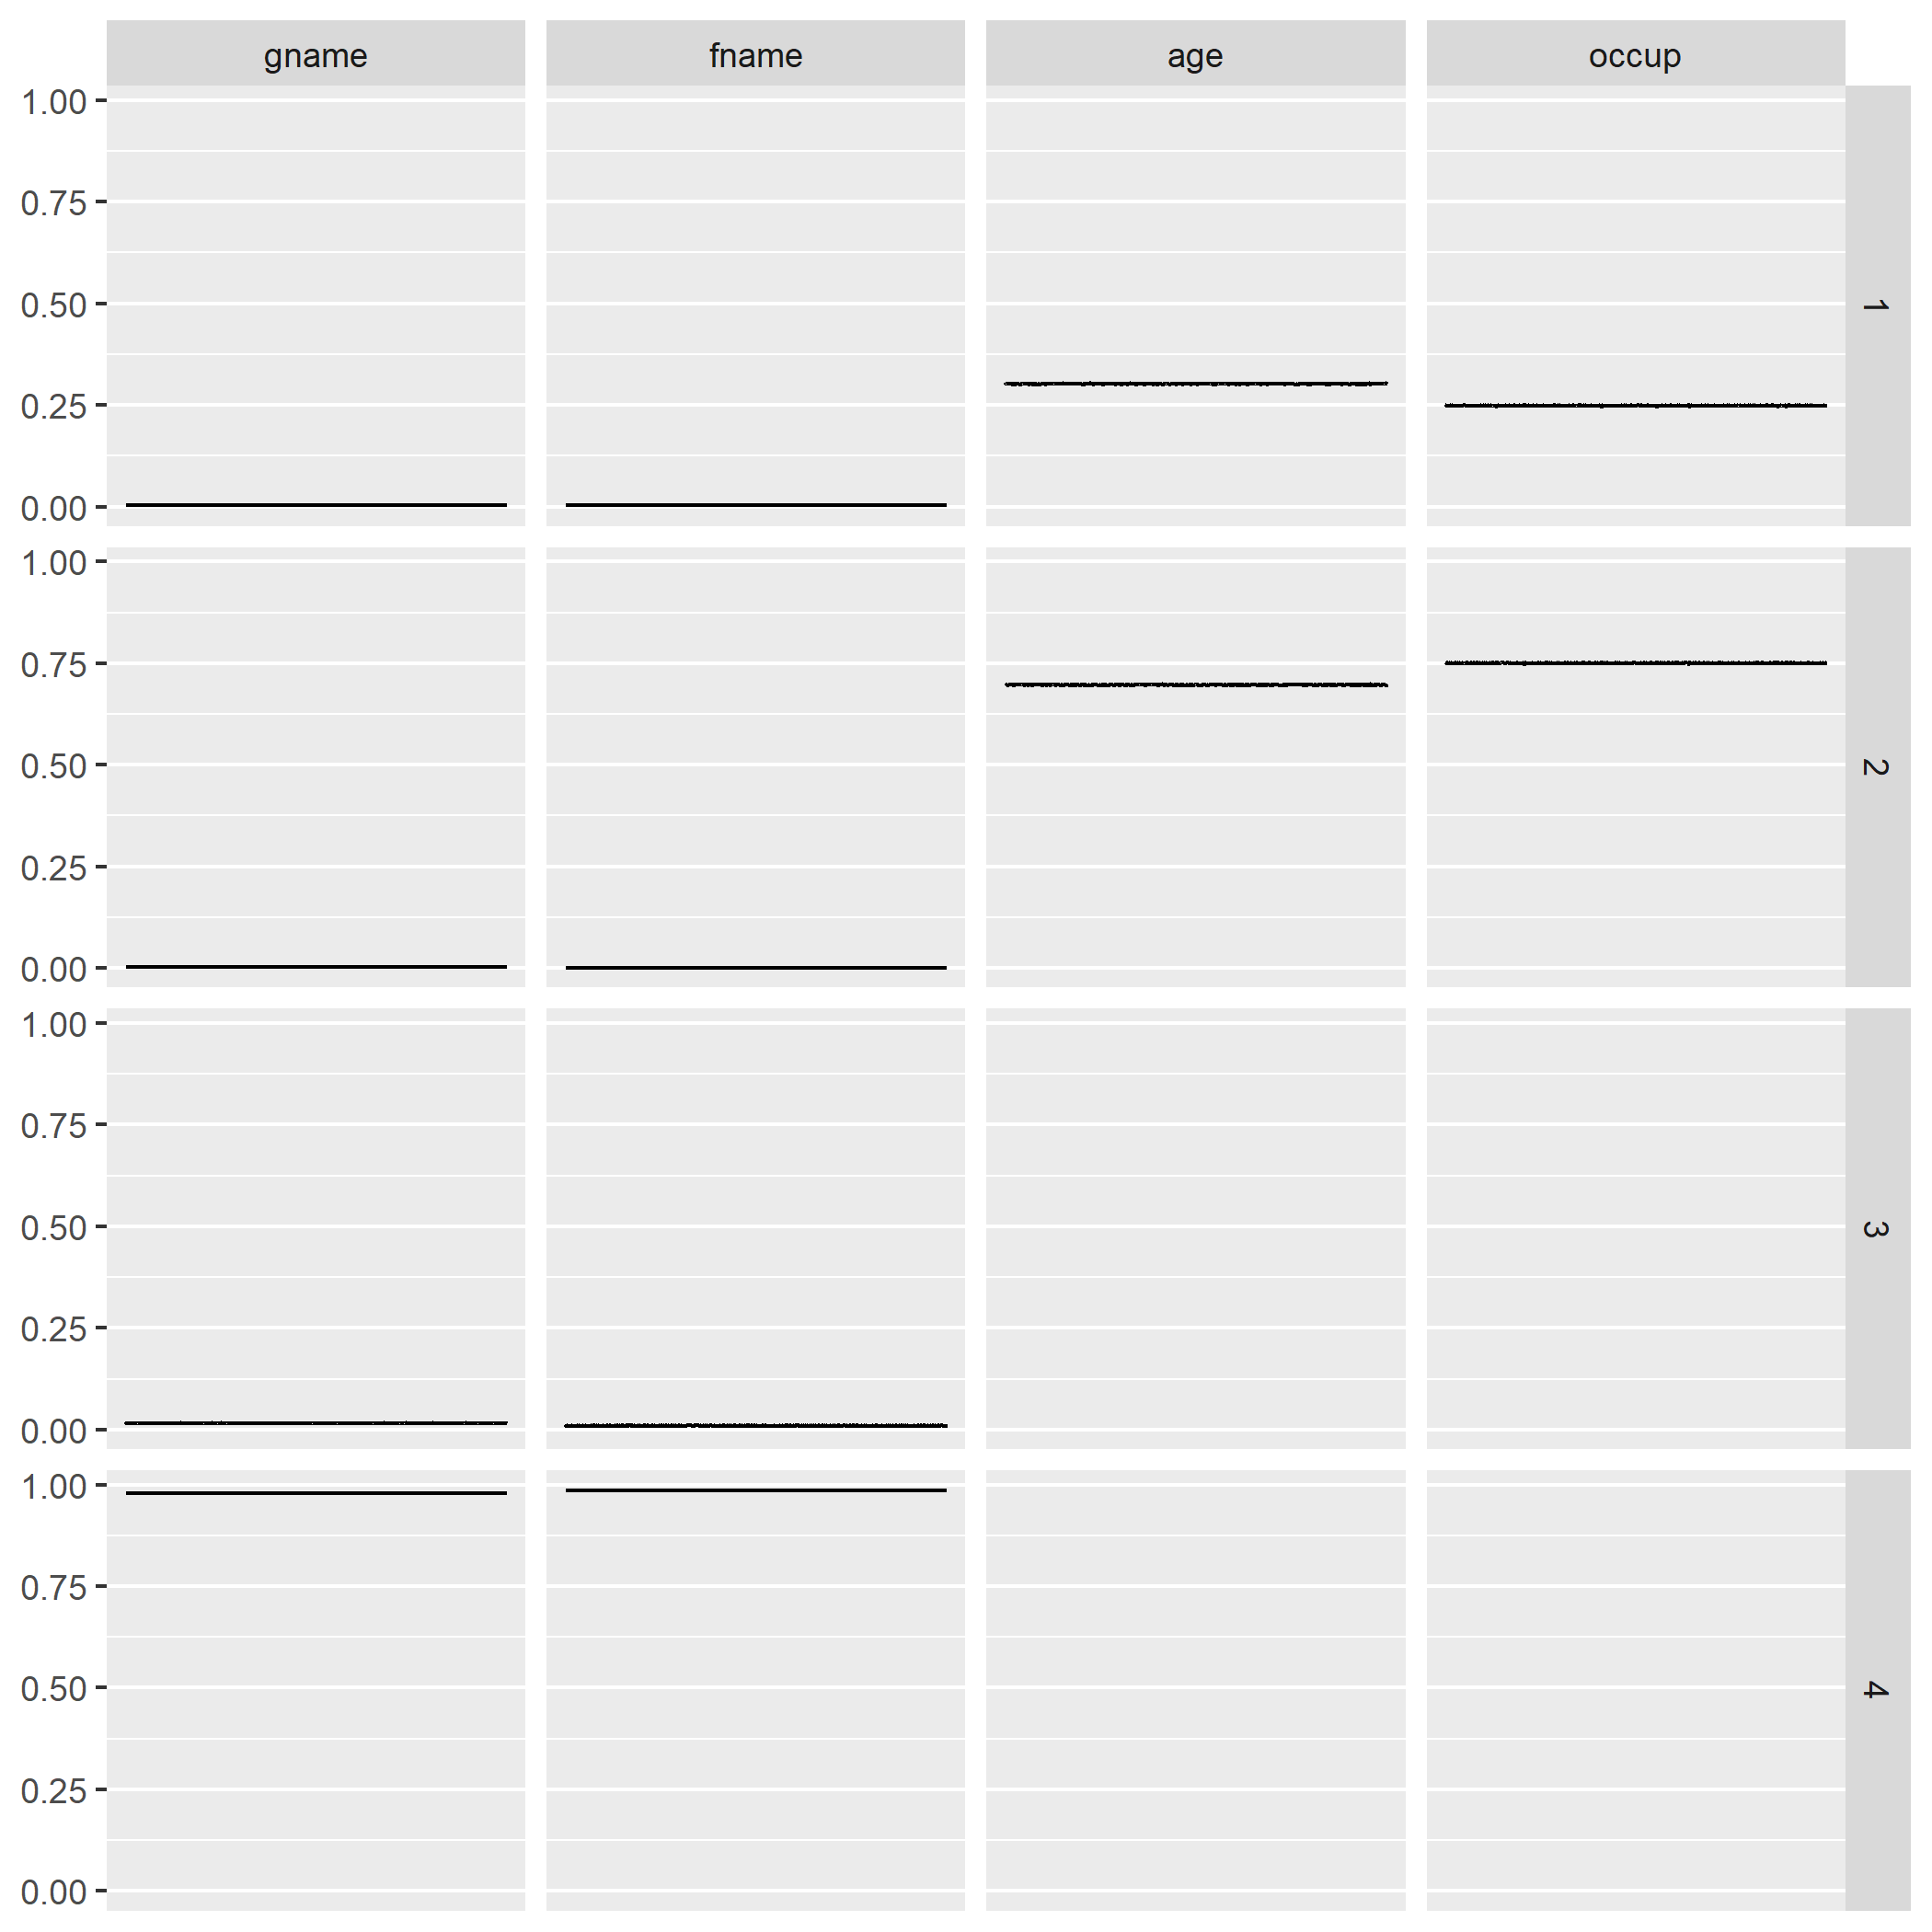
\includegraphics[width=0.6\textwidth]{../notes/figures/sim_u_trace} 
			\caption{Representative traceplot of $\bm{u}$ parameters from simulation study in Section \ref{accuracy} in the main text.}\label{fig:sim_u_trace}
		\end{center}
	\end{figure}

\clearpage

	\hypertarget{partial}{%
	\section{Accuracy under Partial Estimates}\label{partial}}

In this section, we repeat the simulation study in Section \ref{accuracy} in the main text, allowing for clerical review rather than forcing all records to have or not have links.  Specifically, by leaving $\theta_{10} = \theta_{01} = 1$ and $\theta_{11} = 2$, but setting $\theta_R = 0.1$, we allow the model to decline to decide a match for certain records, with nonassignment being 10\% as costly as a false match. In this context, we are no longer focused on finding all true matches, but rather protecting against false matches. Thus, instead of recall, we use the negative predictive value (NPV), defined as the proportion of non-links that are actual nonmatches. Mathematically, $\text{NPV} = \sum_{j=1}^{n_B} I(\hat{Z}_j = Z_j = n_A + j)$/$\sum_{j=1}^{n_B} I(\hat{Z}_j = n_A + j)$. We continue to use the precision, which is renamed the positive predictive value (PPV) in this context. Lastly, we also examine the rejection rate (RR), or how often the model declines to make a linkage decision, defined as RR = $\sum_{j=1}^{n_B} I(\hat{Z}_j = R)/n_B$. To convey this information alongside NPV and PPV, for which values close to 1 indicate strong performance, we report the decision rate (DR), defined as DR = $1 - RR$.

In Figure \ref{fig:sadinle_simulation_partial}, we see that \texttt{fabl} maintains equivalently strong PPV as \texttt{BRL} across all linkage settings. However, with high amounts of error, and thus fewer accurate and discerning fields of information, the rejection rate under \texttt{fabl} rises, leading to a decrease in NPV. Since \texttt{fabl} does not remove previously matched records from consideration for a new record, posterior probabilities of matches at times can be split across more records; in contrast, \texttt{BRL} is able to maintain higher confidence in matches in this setting. If one wishes to use partial estimates, \texttt{fabl} will possibly leave more linkages for the modeler to match by hand than would be left under \texttt{BRL}, but the decisions made by each method should have nearly equal accuracy. 



\begin{figure}
	\begin{center}
		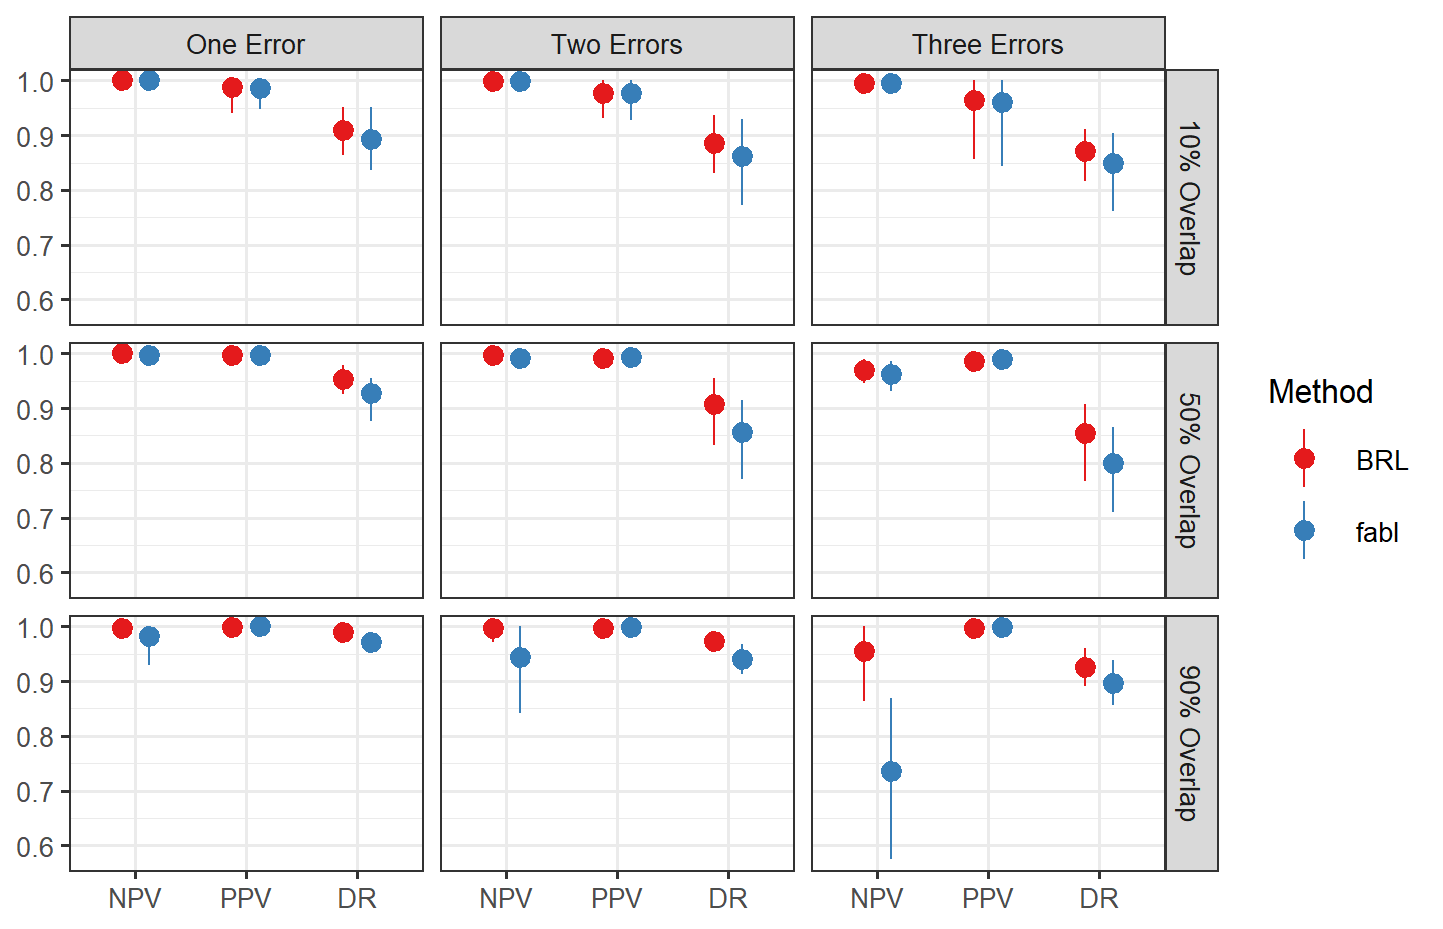
\includegraphics[width=0.99\textwidth]{../notes/figures/sadinle_sim_plot_partial2} 
		\caption{Negative predictive value (NPV), positive predictive value (PPV), and decision rate (DR) on data files in the simulation in Supplement \ref{partial}. We see poorer performance for \texttt{fabl} only in situations with high overlap.}
		\label{fig:sadinle_simulation_partial}
	\end{center}
\end{figure}

\clearpage

	\hypertarget{appendix-speed}{%
	\section{Additional Speed Simulation Study}\label{app:appendix-speed}}
	Figures \ref{fig:app-speed1} and \ref{fig:app-speed2} illustrate that different constructions of the comparison vectors lead to similar speed gains. We replicate the speed study of Section \ref{speed} in the main text under different settings. Here, we use four fields of comparison, each with three possible levels of agreement, resulting in $3^4 = 81$ possible patterns. The $\bm{m}$ and $\bm{u}$ parameters for this simulation are shown in Table \ref{Tab:distributions_2}.
	
		\begin{table}[h]
		\centering
		\begin{tabular}{llll|lll}
			\multicolumn{1}{c}{ } & \multicolumn{3}{c}{$\bm{m}$} & \multicolumn{3}{c}{$\bm{u}$} \\
			\cline{2-4} \cline{5-7}
			& Agree & Partial & Disagree & Agree & Partial & Disagree \\
			\hline
			Feature 1 & $\frac{9}{10}$ & $\frac{9}{100}$  & $\frac{1}{100}$ & $\frac{1}{100}$ &  $\frac{3}{100}$ & $\frac{96}{100}$ \\ 
			Feature 2 & $\frac{9}{10}$ & $\frac{9}{100}$  & $\frac{1}{100}$ & $\frac{1}{100}$ &  $\frac{3}{100}$ & $\frac{96}{100}$ \\ 
			Feature 3 & $\frac{9}{10}$ & $\frac{9}{100}$  & $\frac{1}{100}$ & $\frac{1}{100}$ &  $\frac{3}{100}$ & $\frac{96}{100}$ \\ 
			Feature 4 & $\frac{9}{10}$ & $\frac{9}{100}$  & $\frac{1}{100}$ & $\frac{1}{100}$ &  $\frac{3}{100}$ & $\frac{96}{100}$ \\ 
			\hline
		\end{tabular}
		\caption{Probabilities used for $\bm{m}$ and $\bm{u}$ distributions in simulation study in Supplement~\ref{app:appendix-speed}.}\label{Tab:distributions_2}
	\end{table}
	


	\begin{figure}[h]
	\centering
	\begin{subfigure}{.5\textwidth}
		\centering
		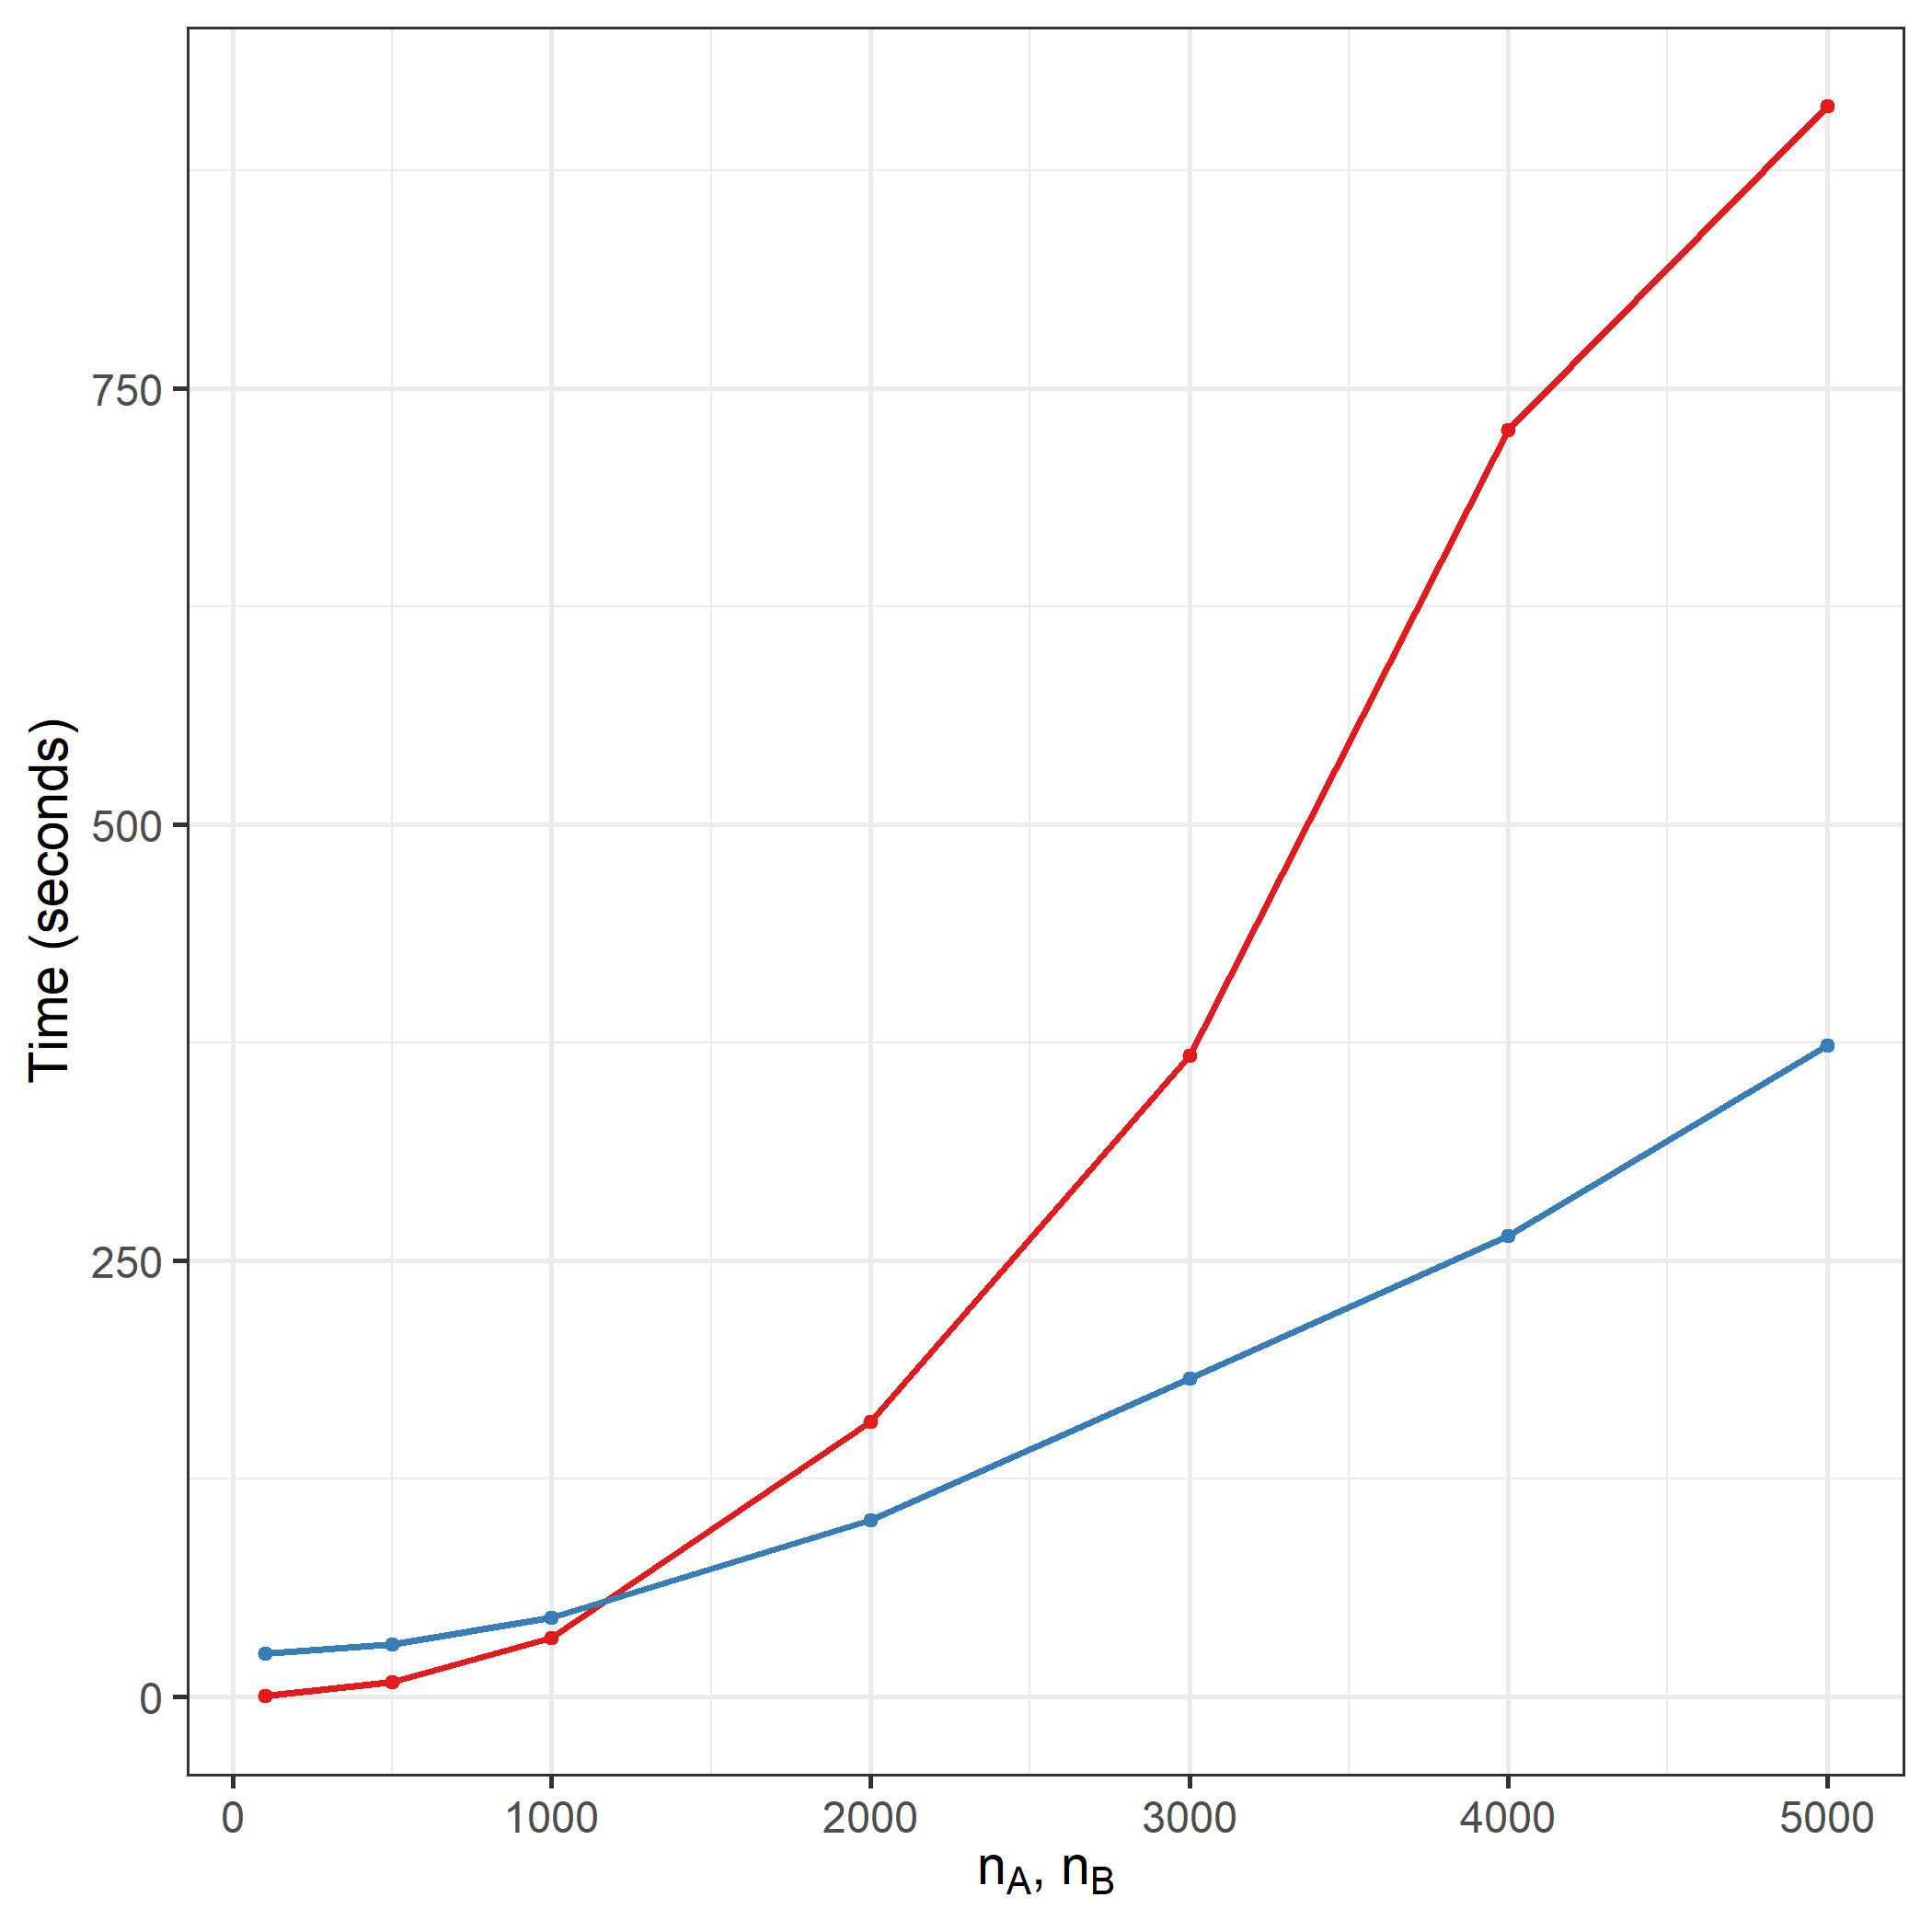
\includegraphics[width=0.95\textwidth]{../notes/figures/sadinle_speed_plot2_new}
		\caption{}
		\label{fig:app-speed1}
	\end{subfigure}%
	\begin{subfigure}{.5\textwidth}
		\centering
		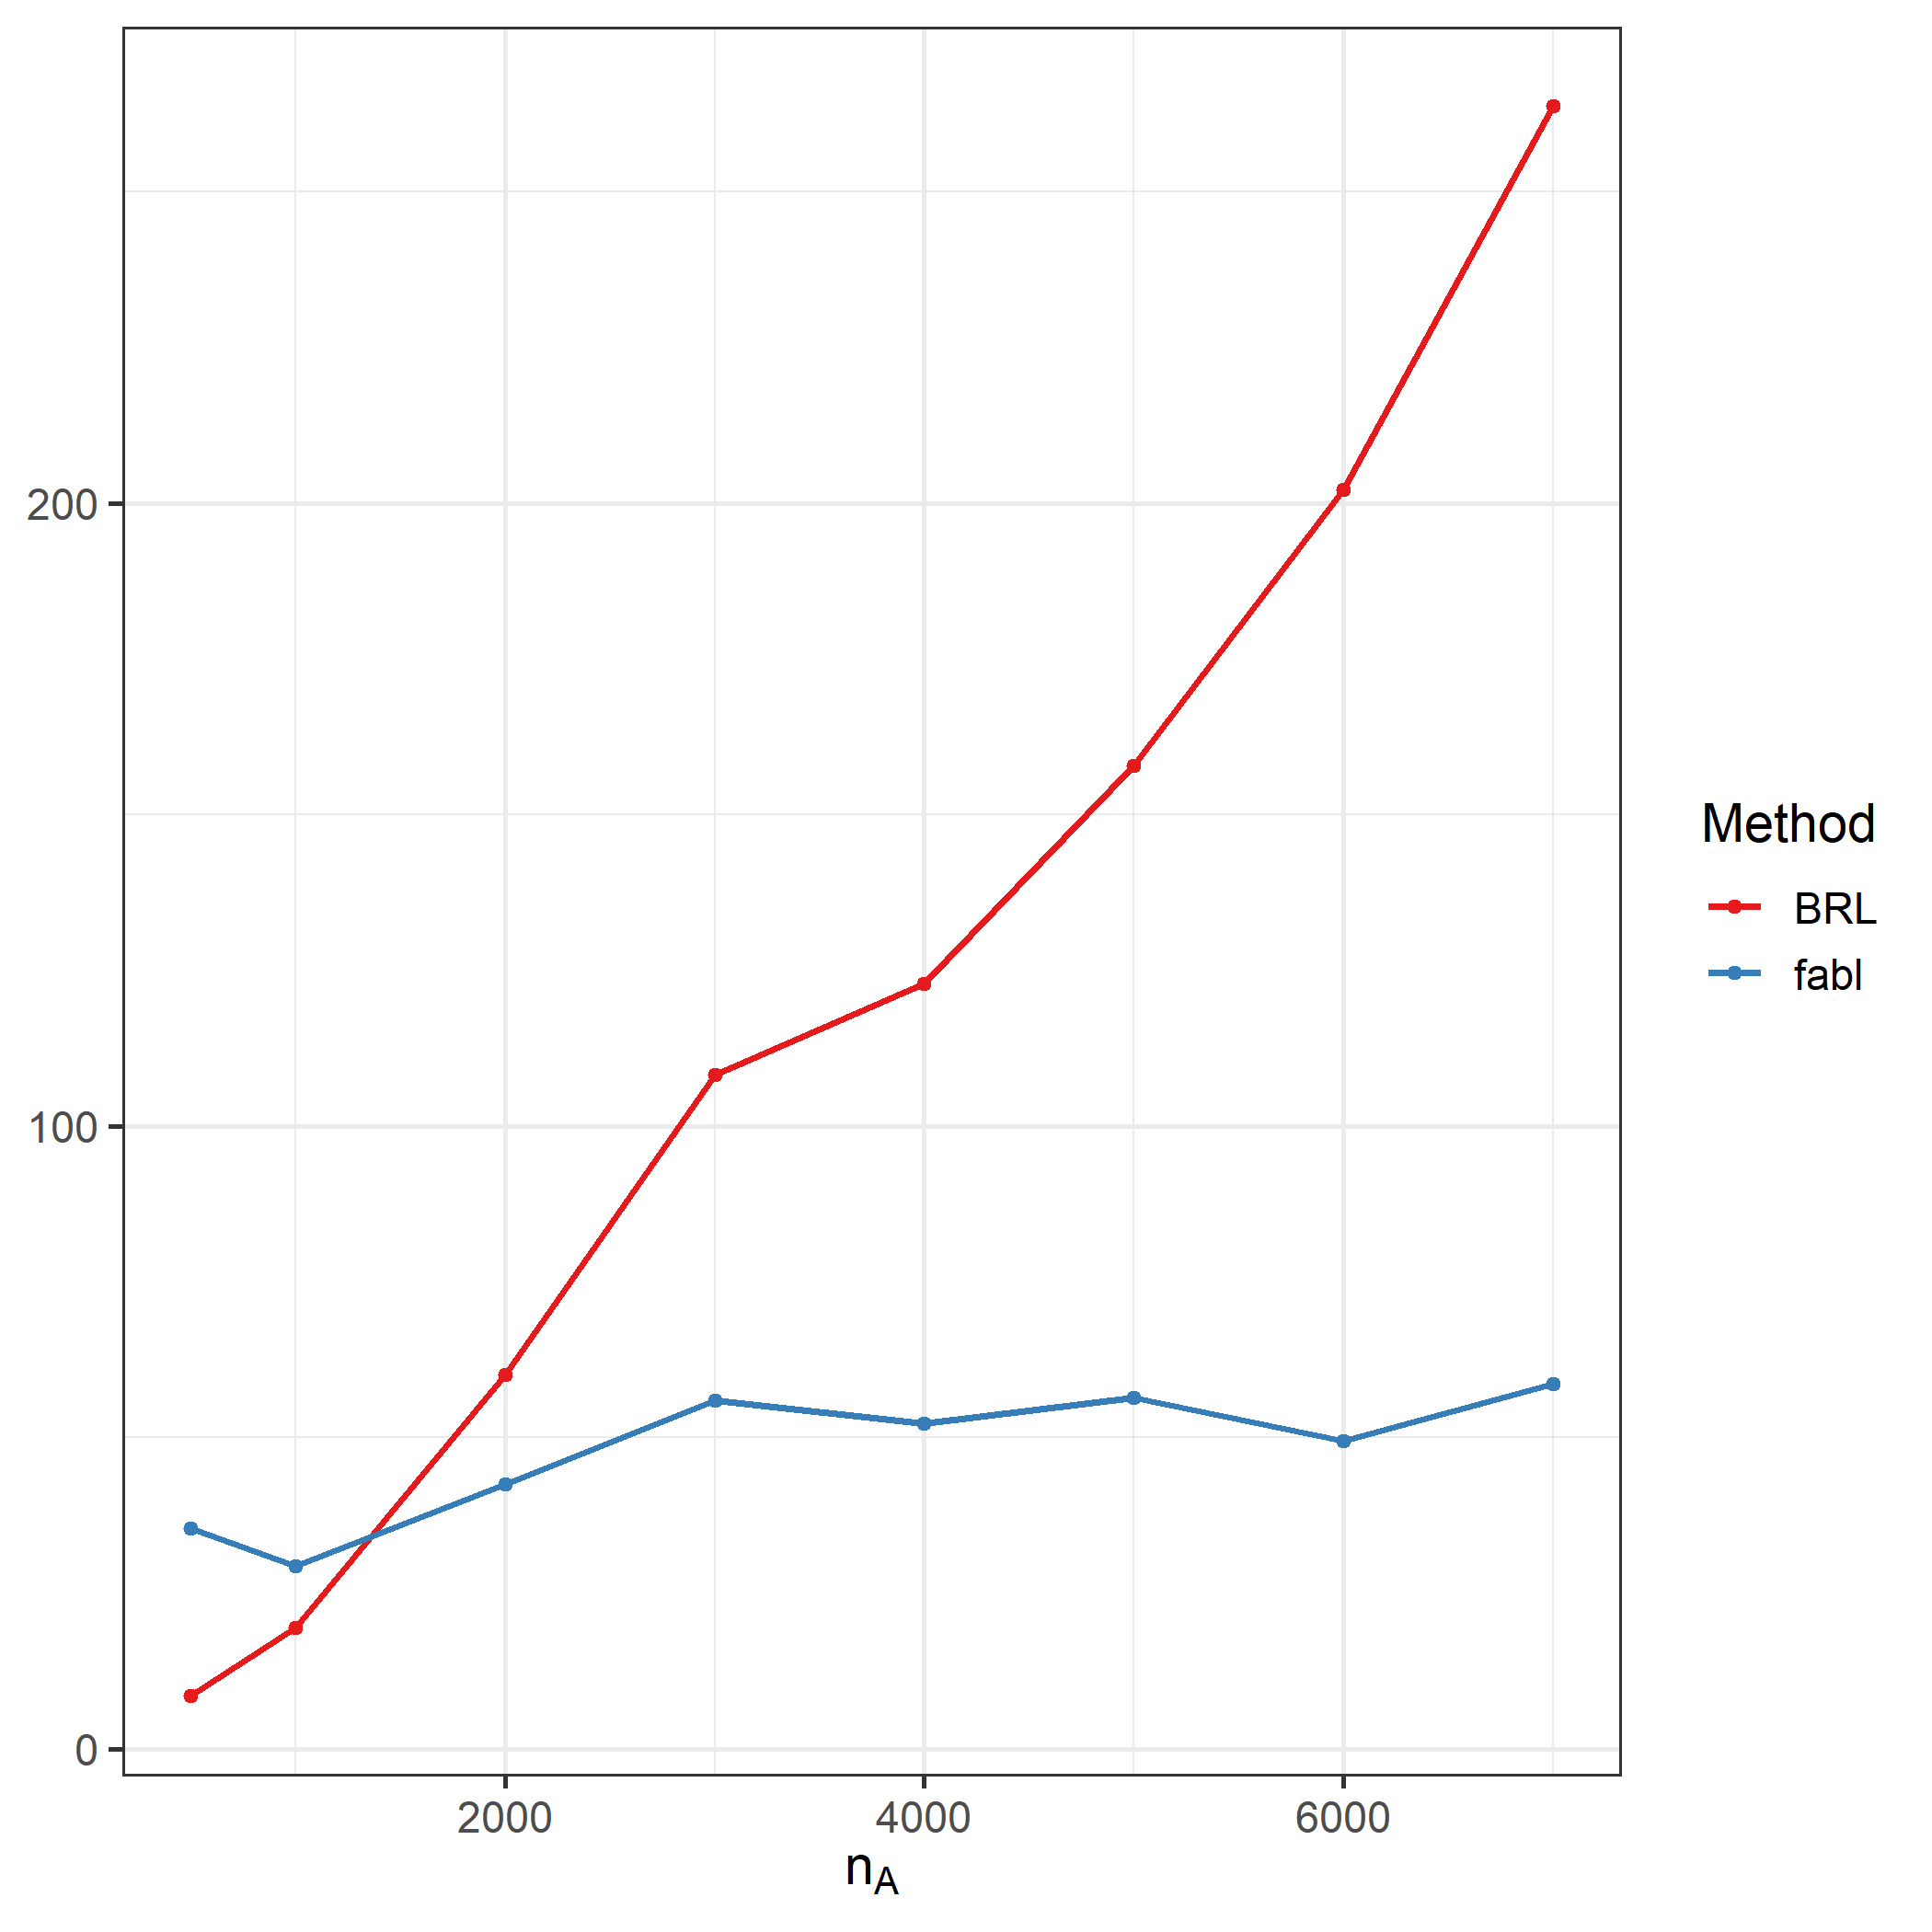
\includegraphics[width=0.95\textwidth]{../notes/figures/speed_plot_fixed_nB2_new} 
		\caption{}
		\label{fig:app-speed2}
	\end{subfigure}
	\caption{Run-time for \texttt{BRL} and \texttt{fabl} to run 1000 Gibbs iterations in simulations described in Supplement \ref{app:appendix-speed}. In (\ref{fig:app-speed1}), both $n_A$ and $n_B$ are increasing. We see quadratic growth in \texttt{BRL} and linear growth in \texttt{fabl}. In (\ref{fig:app-speed2}), only $n_A$ only is increasing. We see linear growth in \texttt{BRL} and approximately constant run-time in \texttt{fabl}.}
	\label{fig:app-speed_sims}
\end{figure}

\clearpage

	\hypertarget{appendix-es}{%
		\section{Traceplots for El Salvador Case Study}\label{app:appendix-es}}
	


    \begin{figure}[h!]
	\centering
	\begin{subfigure}[b]{0.475\textwidth}
		\centering
		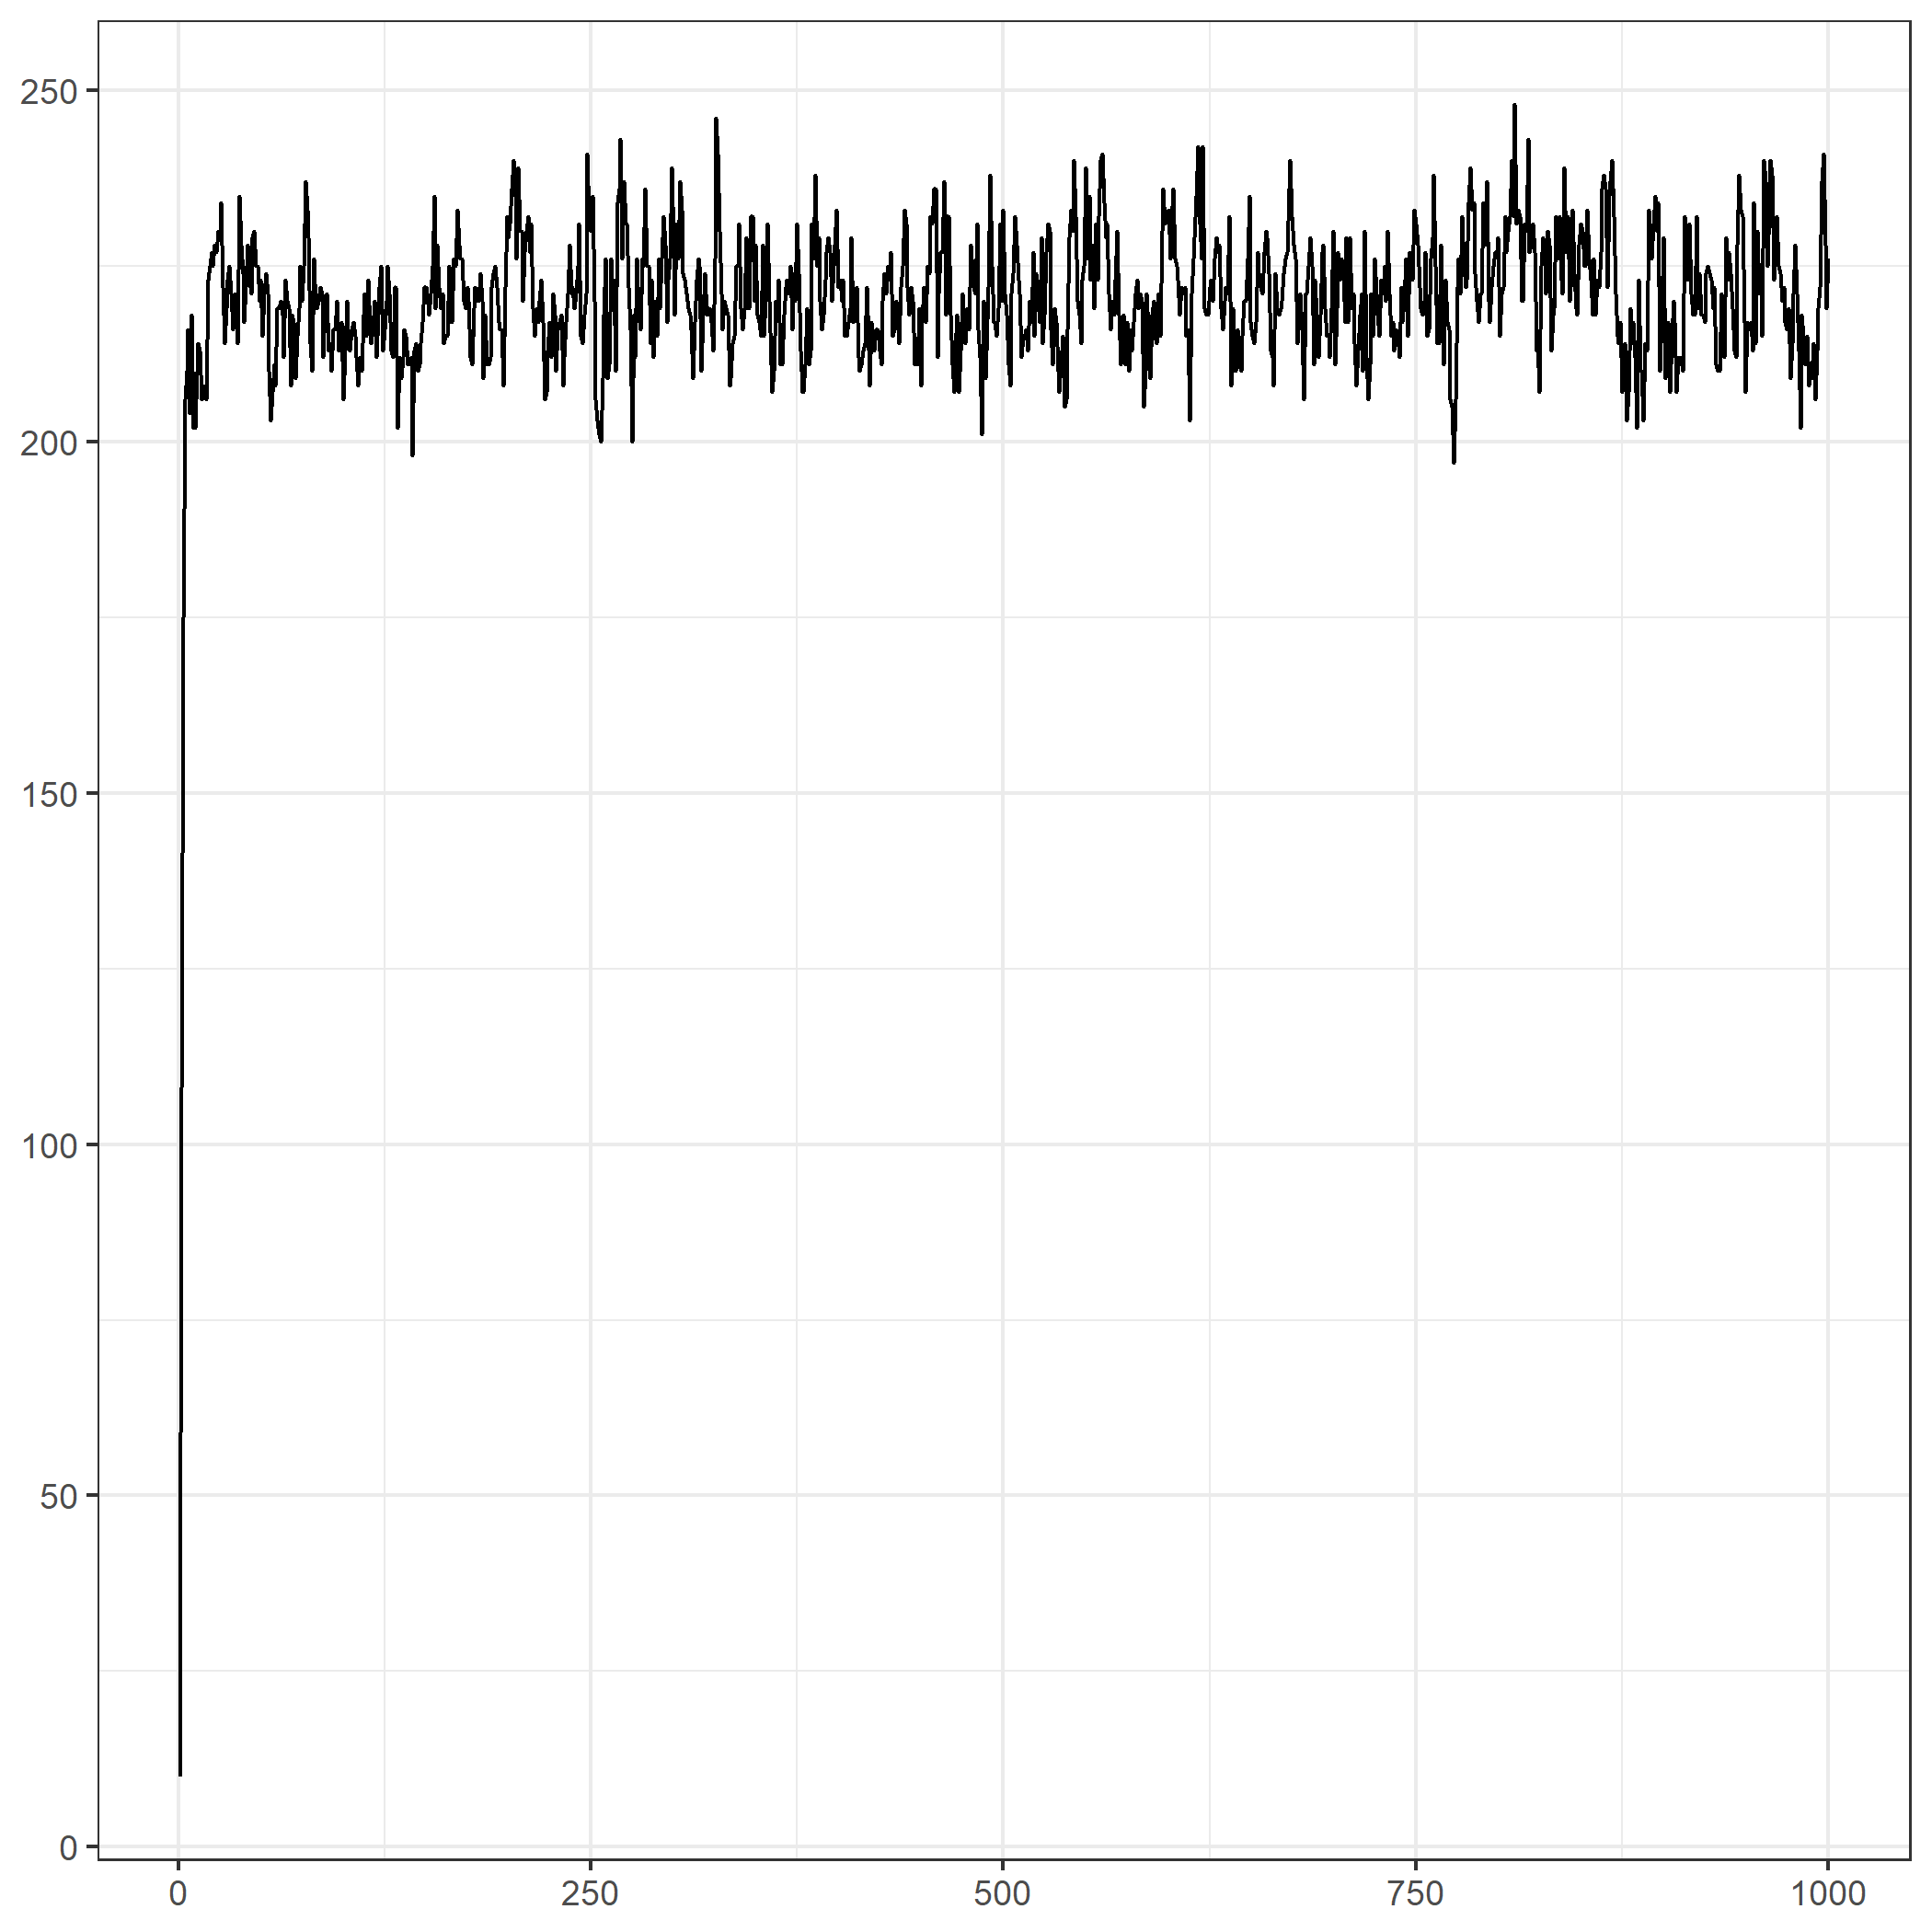
\includegraphics[width=0.975\textwidth]{../notes/figures/el_salvador/overlap_trace} 
		\caption{Traceplot for overlap between files.}    
		\label{fig:overlap_trace}
	\end{subfigure}
	\hfill
	\begin{subfigure}[b]{0.475\textwidth}  
		\centering 
		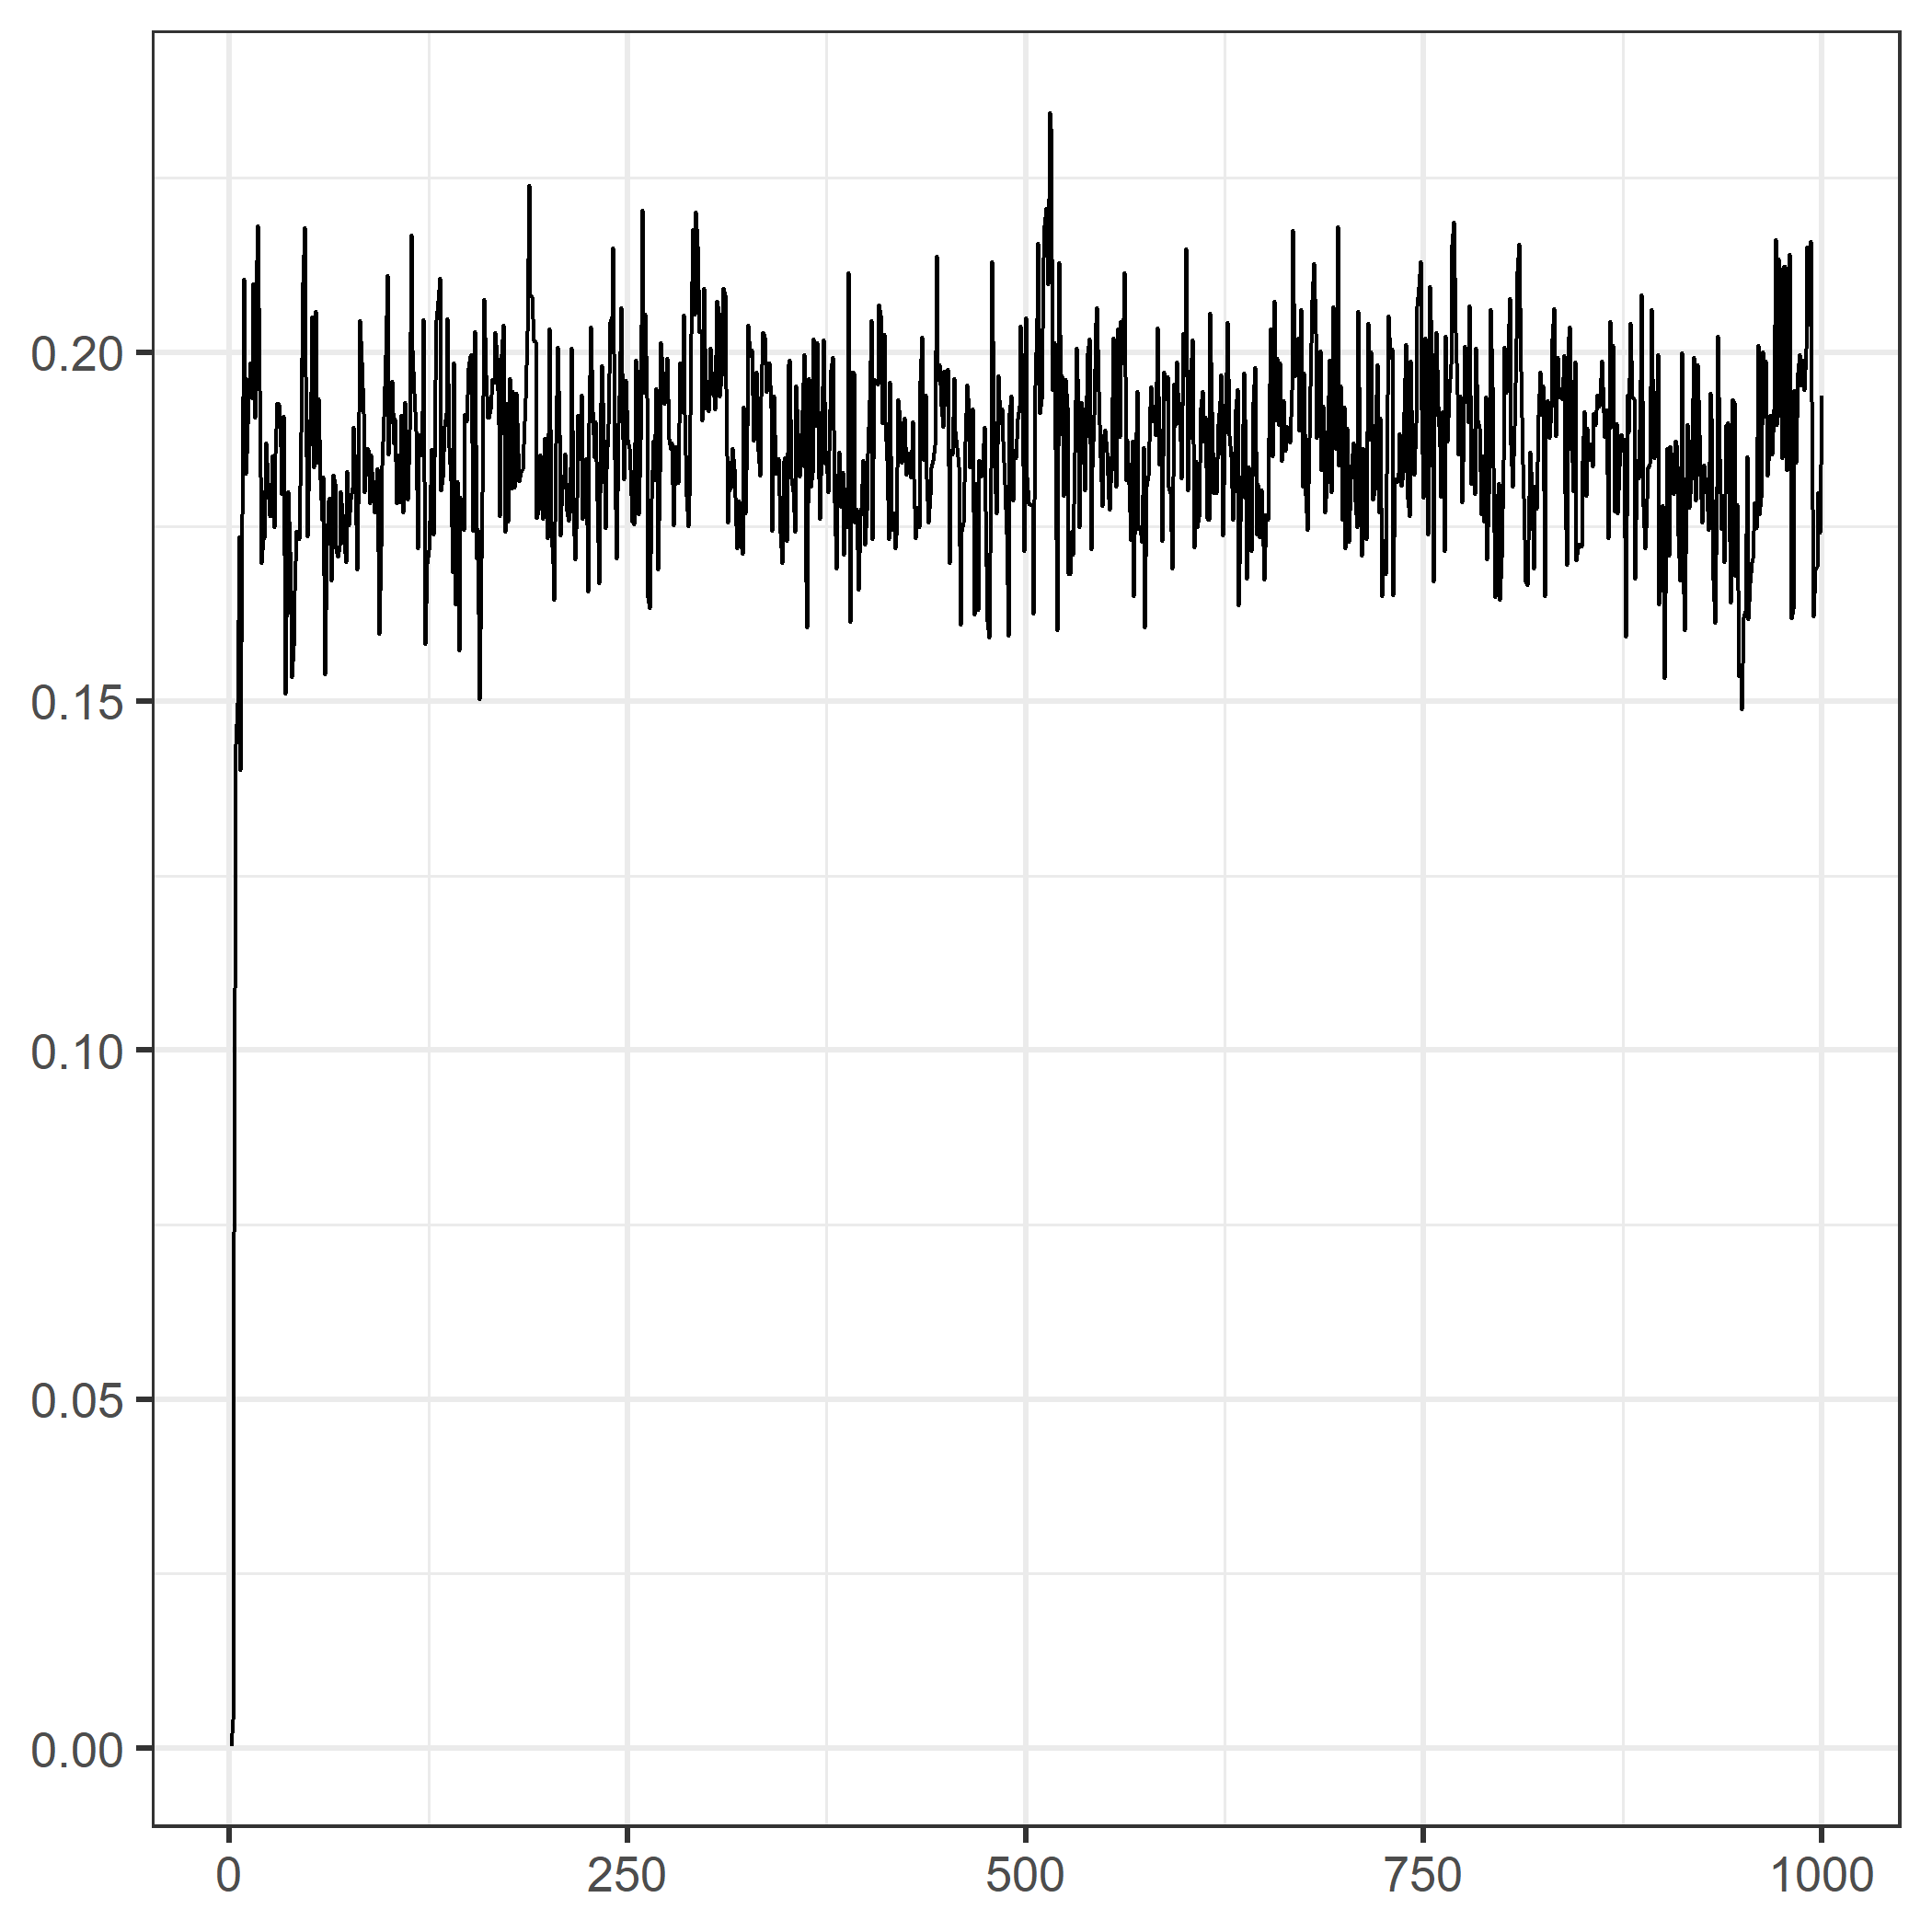
\includegraphics[width=0.975\textwidth]{../notes/figures/el_salvador/pi_trace} 
		\caption{Traceplot for $\pi$.}  
		\label{fig:pi_trace}
	\end{subfigure}
	\vskip\baselineskip
	\begin{subfigure}[b]{0.475\textwidth}   
		\centering 
		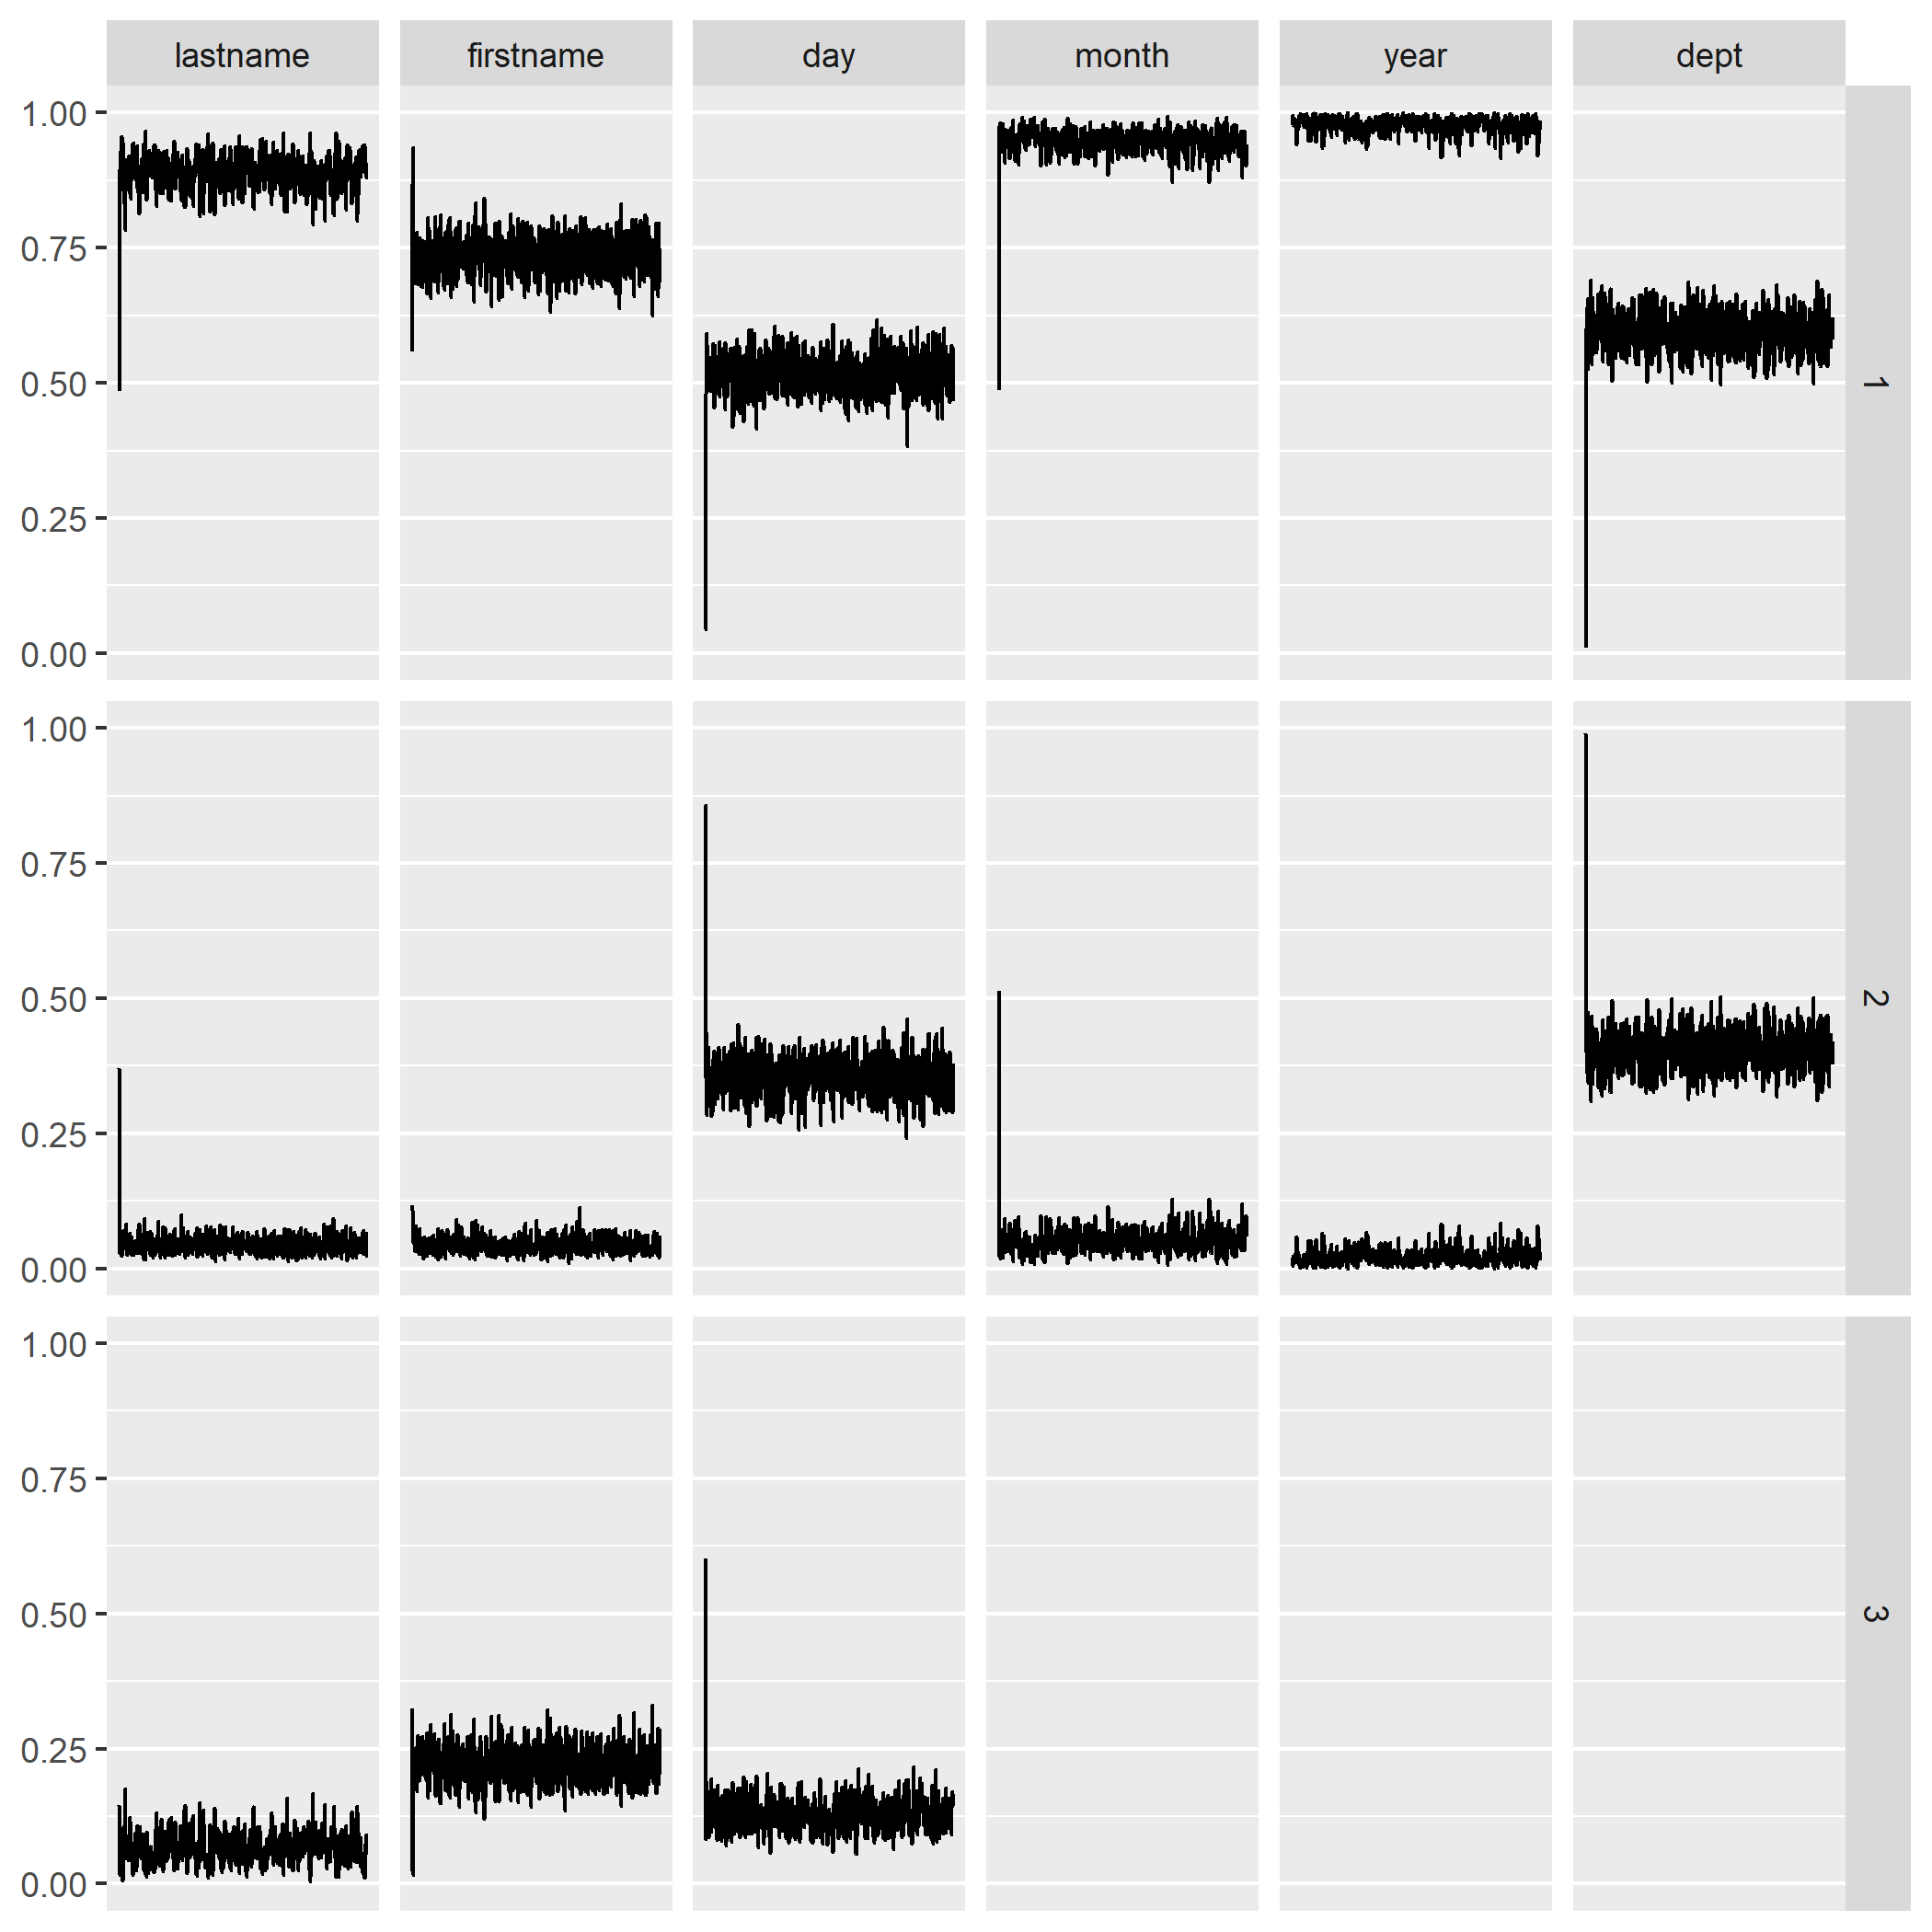
\includegraphics[width=0.975\textwidth]{../notes/figures/el_salvador/m_trace} 
		\caption{Traceplot for $\bm{m}$ parameters.}   
		\label{fig:m_trace}
	\end{subfigure}
	\hfill
	\begin{subfigure}[b]{0.475\textwidth}   
		\centering 
		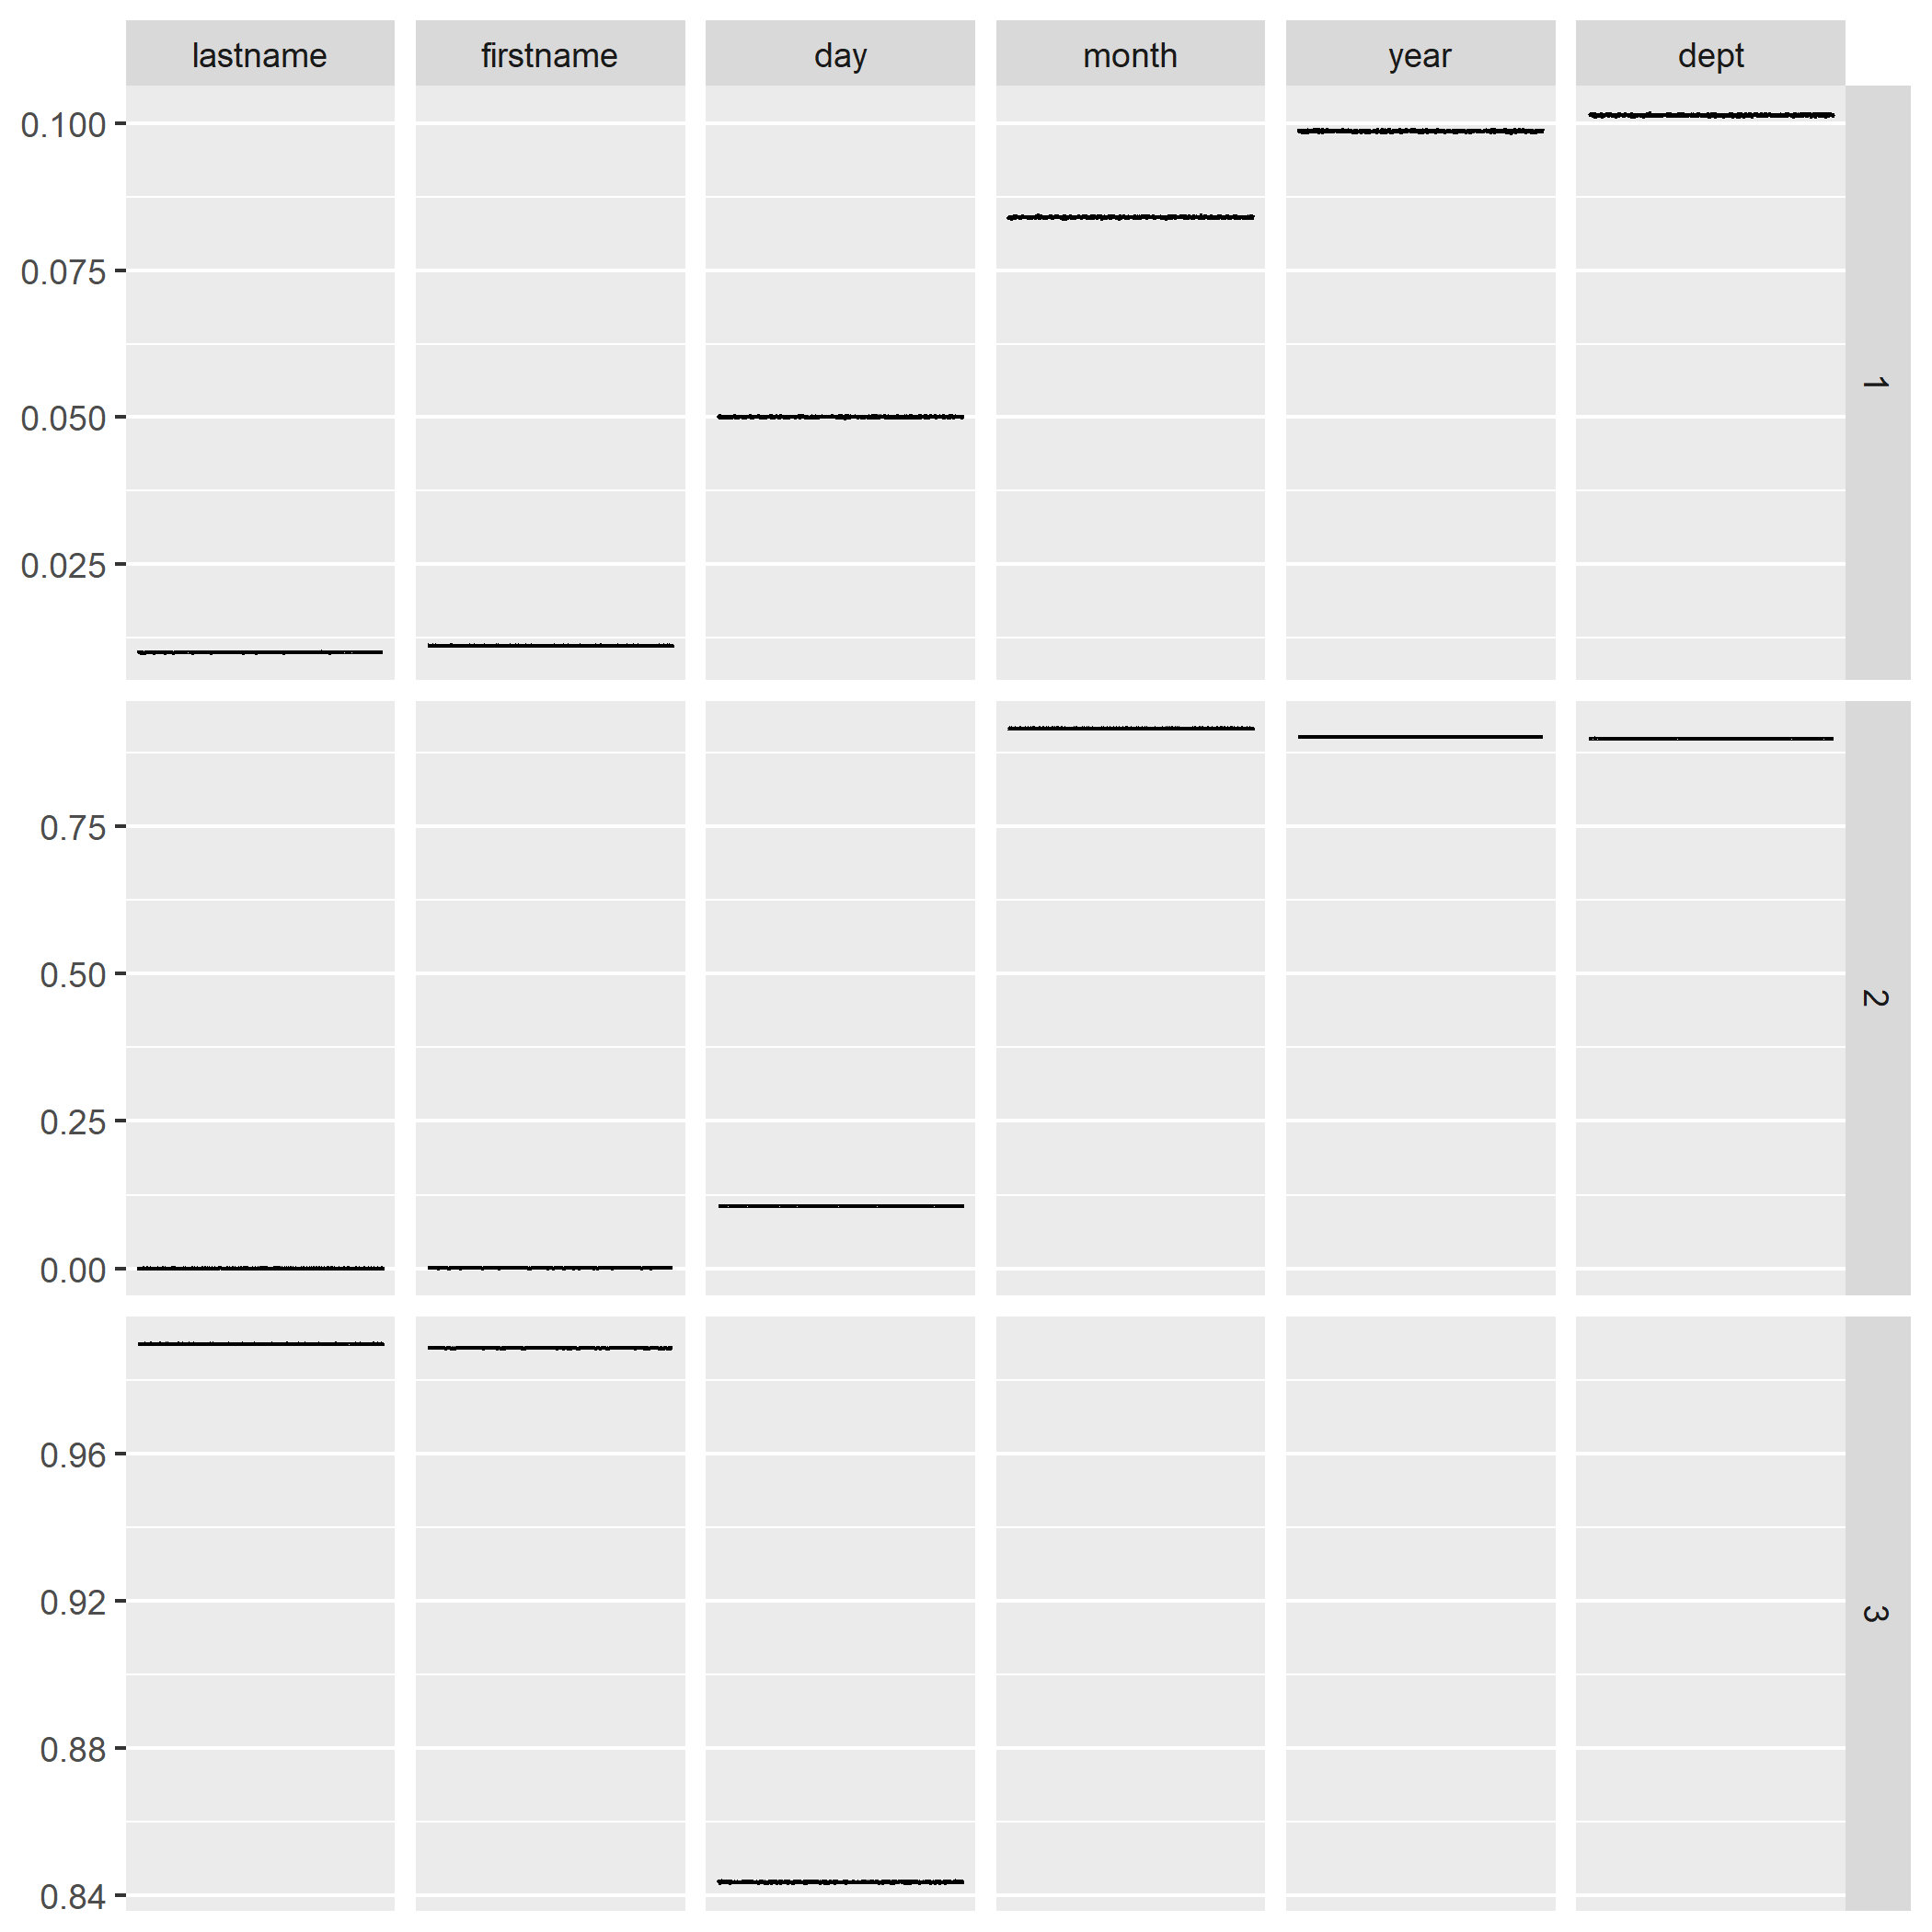
\includegraphics[width=0.975\textwidth]{../notes/figures/el_salvador/u_trace} 
		\caption{Traceplot for $\bm{u}$ parameters.}
		\label{fig:u_trace}
	\end{subfigure}
	\caption{Traceplots for parameters of interest in El Salvador case study in Section \ref{el_salvador} in the main text.}
	\label{fig:el_salvador_trace}
\end{figure}
\end{document}

%\bibliographystyle{jasa}
%	\bibliography{fabl}

\end{document}


	